\documentclass[10pt,a4paper]{book}
\usepackage[utf8]{inputenc}
\usepackage{amsmath,amssymb,amsthm}
\usepackage{enumitem}
\usepackage{geometry}
\usepackage{graphicx}
\usepackage{hyperref}
\usepackage{tikz}
\usetikzlibrary{circuits.logic.US, positioning, arrows}
\usepackage{bussproofs}
\usepackage{makeidx}
\makeindex
\usepackage[thinlines]{easytable}
\usepackage{array}
\usepackage{nicematrix,tikz}
\usetikzlibrary{arrows.meta,ext.paths.ortho} % for "r-lr"
\usepackage{mfirstuc}
\usepackage{twemojis}
\usepackage{fontspec}
\usepackage{parskip}
\usepackage{amssymb}
\usepackage{emptypage}



\usepackage[outerline=false]{fitch}



\let\oldemptyset\emptyset
\let\emptyset\varnothing


\linespread{1.05} % Slightly increases line height



\newtheorem{undefined}{Undefined}[section]
\newtheorem{definition}{Definition}[section]
\newtheorem{theorem}{Theorem}[section]
\newtheorem{lemma}{Lemma}[section]
\newtheorem{axiom}{Axiom}[section]
\newtheorem{example}{Example}[section]
\newtheorem{exercise}{Exercise}[section]
\newtheorem{Rule}{Rule}[section]
\newtheorem{Attention}{Attention}[section]
\newtheorem{observation}{Observation}[section]
\newtheorem{colloraly}{Colloraly}[section]
\makeatletter
\renewcommand{\arraystretch}{1.44} % 2x standard row height


\newcommand*{\blankpage}{
  \vspace*{\fill}
  \begin{center}
    \textit{This page intentionally left blank.}
  \end{center}
  \vspace*{\fill}
}
\renewcommand*{\cleardoublepage}{%
  \clearpage
  \if@twoside
    \ifodd\c@page
    \else
      \blankpage
      \thispagestyle{empty}
      \newpage
      \if@twocolumn\hbox{}\newpage\fi
    \fi
  \fi
}
\makeatother



\begin{document}

\frontmatter
\title{\textbf{\Huge Logic}}
\author{\Large Aria Ruler(Forouzandeh)}
\date{\today}
\maketitle

\tableofcontents

\mainmatter

\chapter{Atomes}
\section{Basic tools}

we start the book by building logic step by step.block by block in first it
might seem a little annoying but I advice you to be patient.book will show its
power soon. like euclidian geometry this book has undefined concepts. I tried
to explain them for you to understand.but they don't have any definition.
\begin{undefined}
    \textbf{Urelements} are the most fundamental entities in a logical.
    They cannot be constructed, defined, or described in terms of other things.
    Their existence is primitive—accepted without internal structure or relational properties.
    Urelements simply are.
\end{undefined}

In this book, we will denote individual urelements using lowercase letters such
as $a$, $b$, $c$,$...$

\begin{undefined}
    \textbf{Type} parallel lines used to show that an object exists
    (you will undrestnd what is object soon.)
    (we will show you how to use them).

    \begin{tikzpicture}
        % Vertical lines
        \draw (0,0) -- (0,4);
        \draw (1,0) -- (1,4);
        \draw (2,0) -- (2,4);
        \draw (3,0) -- (3,4);
        % Labels between lines
        \node at (-0.5,3) {1.};
        \node at (-0.5,2) {2.};
        \node at (-0.5,1) {3.};
        \node at (0.2,3) {$a$};
        \node at (1.2,2) {$b$};
        \node at (2.2,1) {$c$};
    \end{tikzpicture}
\end{undefined}

\begin{Rule}
    \textbf{fusion} it's the Rule that explain how sets made.
    (this rule is schema.it means it works everywhere for every object.)

    \begin{tikzpicture}
        % Vertical lines
        \draw (0,0) -- (0,5);
        \draw (1,0) -- (1,5);
        % \draw (1.5,3.6) -- (-0.1,3.6) -- (-0.1,0.5) -- (1.5,0.5);
        % Labels between lines
        \node at (-0.5,4) {$m.$};
        \node at (-0.6,2) {$m+n.$};
        \node at (-0.5,1) {$o.$};
        \node at (0.2,4) {$a_{0}$};
        \node at (0.2,3) {$\vdots$};
        \node at (0.2,2) {$a_{n}$};
        \node at (2,1) {$\{a_{0} , a_{1}... a_{n}\}$};
    \end{tikzpicture}
\end{Rule}

\begin{undefined}
    \textbf{Set} we can't say what exactly sets are but we know sets can be made by fusion
    (from now we denote sets with uppercase letters).
\end{undefined}

\begin{definition}
    \textbf{Object} urelements and sets.(we write obj instead of object).
\end{definition}

\begin{Rule}
    \textbf{fission} it show us how to break an obj.
    (this rule is scheme it means it works everywhere for every obj.)

    \begin{tikzpicture}
        % Vertical lines
        \draw (0,-1) -- (0,4);
        \draw (1,-1) -- (1,4);
        % \draw (1.5,3.6) -- (-0.1,3.6) -- (-0.1,0.5) -- (1.5,0.5);
        % Labels between lines
        \node at (-0.5,3) {$o.$};
        \node at (-0.5,2) {$m.$};
        \node at (-0.6,0) {$m+n.$};
        \node at (2,3) {$\{a_{0} , a_{1}... a_{n}\}$};
        \node at (0.2,2) {$a_{0}$};
        \node at (0.2,1) {$\vdots$};
        \node at (0.2,0) {$a_{n}$};
    \end{tikzpicture}

\end{Rule}

\begin{example}
    \textbf{} $\{a,b,c\} /\therefore \{a,b\}$
    (prove if $\{a,b,c\}$ exists then $\{a,c\}$ exists)

    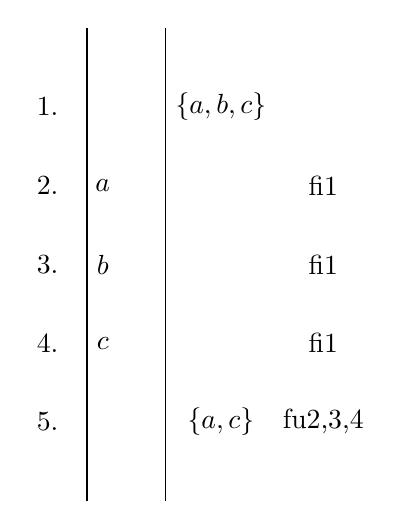
\begin{tikzpicture}
        % Vertical lines
        \draw (0,-2) -- (0,4);
        \draw (1,-2) -- (1,4);
        % \draw (1.5,3.6) -- (-0.1,3.6) -- (-0.1,-1.5) -- (1.5,-1.5);
        % Labels between lines
        \node at (-0.5,3) {1.};
        \node at (-0.5,2) {2.};
        \node at (-0.5,1) {3.};
        \node at (-0.5,0) {4.};
        \node at (-0.5,-1) {5.};
        \node at (1.7,3) {$\{a,b,c\}$};
        \node at (0.2,2) {$a$};
        \node at (3,2) {fi1};
        \node at (0.2,1) {$b$};
        \node at (3,1) {fi1};
        \node at (0.2,0) {$c$};
        \node at (3,0) {fi1};
        \node at (1.7,-1) {$\{a,c\}$};
        \node at (3,-1) {fu2,3,4};
    \end{tikzpicture}

\end{example}

\begin{example}
    \textbf{} $\{a,b\} /\therefore \{b,a\}$

    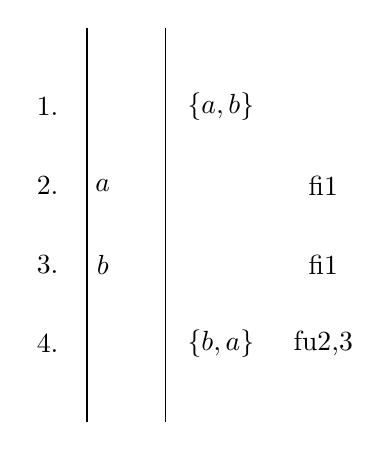
\begin{tikzpicture}
        % Vertical lines
        \draw (0,-1) -- (0,4);
        \draw (1,-1) -- (1,4);
        % \draw (1.5,3.6) -- (-0.1,3.6) -- (-0.1,-0.5) -- (1.5,-0.5);
        % Labels between lines
        \node at (-0.5,3) {1.};
        \node at (-0.5,2) {2.};
        \node at (-0.5,1) {3.};
        \node at (-0.5,0) {4.};
        \node at (1.7,3) {$\{a,b\}$};
        \node at (0.2,2) {$a$};
        \node at (3,2) {fi1};
        \node at (0.2,1) {$b$};
        \node at (3,1) {fi1};
        \node at (1.7,0) {$\{b,a\}$};
        \node at (3,0) {fu2,3};
    \end{tikzpicture}
\end{example}

\begin{Rule}
    \textbf{repetition} you can repeat an obj
    (this rule is scheme it means it works everywhere for every obj.)

    \begin{tikzpicture}
        % Vertical lines
        \draw (0,1.5) -- (0,3.5);
        % \draw (1.5,2.6) -- (-0.1,2.6) -- (-0.1,0.5) -- (1.5,0.5);
        % Labels between lines
        \node at (-0.5,3) {$n.$};
        \node at (-0.5,2) {$m.$};
        \node at (0.2,3) {$a$};
        \node at (0.2,2) {$a$};
        \node at (2.2,2) {rp};
    \end{tikzpicture}
\end{Rule}

\begin{undefined}
    \textbf{Gutter} is a tool to make an object isolated.
    (nothing can get in or out and the focused obj is the first obj in gutter)
    with Gutter we can undrestnd object
    More precisely we denote Gutter like this.

    \begin{tikzpicture}
        \draw (1,0) -- (0,0) -- (0,2) -- (1,2);
    \end{tikzpicture}

\end{undefined}

\begin{Rule}
    \textbf{repetition in Gutter} you can only repeat an obj
    in Gutter once(Gutter isolated obj).

    \begin{tikzpicture}
        % Vertical lines
        \draw (0,1) -- (0,3.5);
        \draw (1.5,2.6) -- (-0.1,2.6) -- (-0.1,1.5) -- (1.5,1.5);
        % Labels between lines
        \node at (-0.5,3) {$n.$};
        \node at (-0.5,2) {$m.$};
        \node at (0.2,3) {$a$};
        \node at (0.2,2) {$a$};
        \node at (2.2,2) {rpg.$n$};
    \end{tikzpicture}
\end{Rule}

\section{ Identity }

\begin{undefined}
    \textbf{identity} $(=)$ one of the basice concepts that talk about two things are the same.
\end{undefined}

\begin{Rule}
    \textbf{$I=$} (this rule is scheme it means it works everywhere for every obj.)

    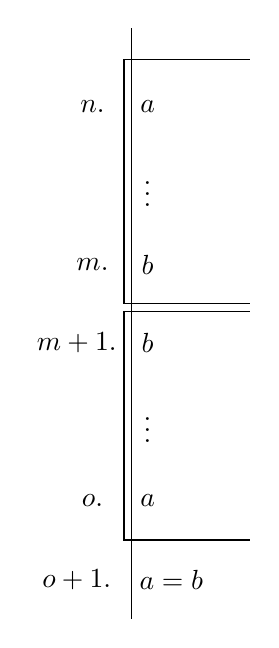
\begin{tikzpicture}
        % Vertical lines
        \draw (0,-1.5) -- (0,6);
        \draw (1.5,5.6) -- (-0.1,5.6) -- (-0.1,2.5) -- (1.5,2.5);
        \draw (1.5,2.4) -- (-0.1,2.4) -- (-0.1,-0.5) -- (1.5,-0.5);
        % Labels between lines
        \node at (-0.5,5) {$n.$};
        \node at (-0.5,3) {$m.$};
        \node at (-0.7,2) {$m+1.$};
        \node at (-0.5,0) {$o.$};
        \node at (-0.7,-1) {$o+1.$};
        \node at (0.2,5) {$a$};
        \node at (0.2,4) {$\vdots$};
        \node at (0.2,3) {$b$};
        \node at (0.2,2) {$b$};
        \node at (0.2,1) {$\vdots$};
        \node at (0.2,0) {$a$};
        \node at (0.5,-1) {$a=b$};
    \end{tikzpicture}

\end{Rule}

\begin{Rule}
    \textbf{$E=$} (this rule is scheme it means it works everywhere for every obj.)

    \begin{tikzpicture}
        % Vertical lines
        \draw (0,0) -- (0,4);
        % Labels between lines
        \node at (-0.5,3) {$n.$};
        \node at (-0.5,2) {$m.$};
        \node at (-0.5,1) {$o.$};
        \node at (0.2,3) {$a$};
        \node at (0.5,2) {$a=b$};
        \node at (0.2,1) {$b$};
        \node at (3,1) {$E= n,m$};

    \end{tikzpicture}

\end{Rule}

\begin{example}
    \textbf{} $a/\therefore a = a$

    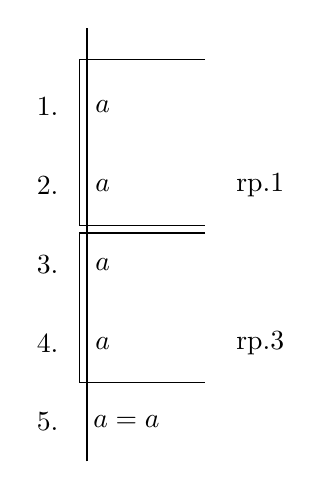
\begin{tikzpicture}
        % Vertical lines
        \draw (0,-1.5) -- (0,4);
        \draw (1.5,3.6) -- (-0.1,3.6) -- (-0.1,1.5) -- (1.5,1.5);
        \draw (1.5,1.4) -- (-0.1,1.4) -- (-0.1,-0.5) -- (1.5,-0.5);
        % Labels between lines
        \node at (-0.5,3) {1.};
        \node at (-0.5,2) {2.};
        \node at (-0.5,1) {3.};
        \node at (-0.5,0) {4.};
        \node at (-0.5,-1) {5.};
        \node at (0.2,3) {$a$};
        \node at (0.2,2) {$a$};
        \node at (2.2,2) {rp.1};
        \node at (0.2,1) {$a$};
        \node at (0.2,0) {$a$};
        \node at (2.2,0) {rp.3};
        \node at (0.5,-1) {$a=a$};
    \end{tikzpicture}

\end{example}

\begin{example}
    \textbf{} $a,b/\therefore \{a,b\} = \{b,a\}$

    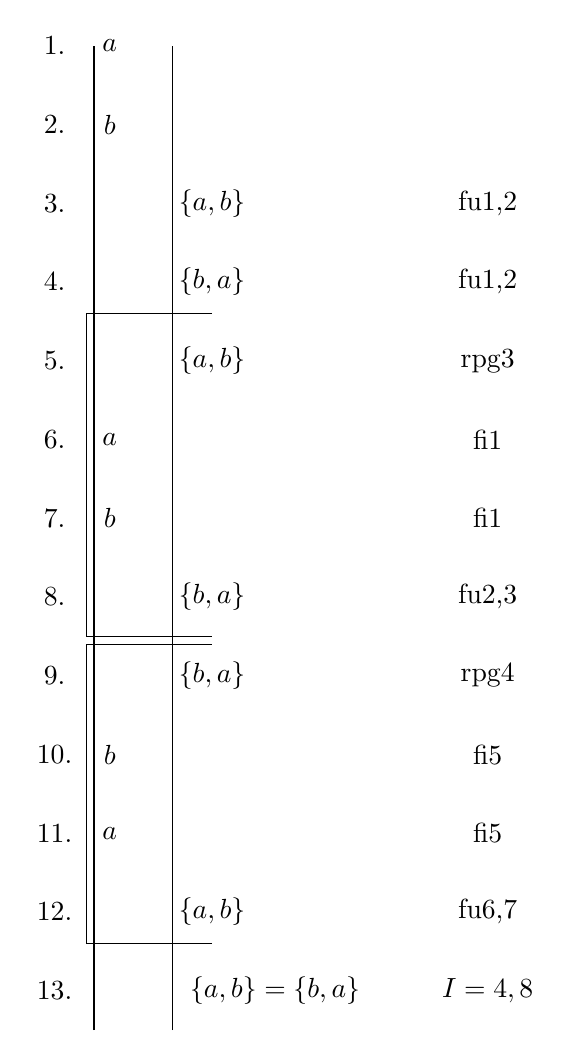
\begin{tikzpicture}
        % Vertical lines
        \draw (0,-5.5) -- (0,7);
        \draw (1,-5.5) -- (1,7);
        \draw (1.5,3.6) -- (-0.1,3.6) -- (-0.1,-0.5) -- (1.5,-0.5);
        \draw (1.5,-4.4) -- (-0.1,-4.4) -- (-0.1,-0.6) -- (1.5,-0.6);
        \node at (-0.5,7) {1.};
        \node at (-0.5,6) {2.};
        \node at (-0.5,5) {3.};
        \node at (-0.5,4) {4.};
        \node at (-0.5,3) {5.};
        \node at(-0.5,2) {6.};
        \node at (-0.5,1) {7.};
        \node at (-0.5,0) {8.};
        \node at(-0.5,-1) {9.};
        \node at (-0.5,-2) {10.};
        \node at (-0.5,-3) {11.};
        \node at (-0.5,-4) {12.};
        \node at (-0.5,-5) {13.};
        \node at (0.2,7) {$a$};
        \node at(0.2,6) {$b$};
        \node at (1.5,5) {$\{a,b\}$};
        \node at (5,5) {fu1,2};
        \node at(1.5,4) {$\{b,a\}$};
        \node at (5,4) {fu1,2};
        \node at (1.5,3) {$\{a,b\}$};
        \node at (5,3) {rpg3};
        \node at (0.2,2) {$a$};
        \node at (5,2) {fi1};
        \node at(0.2,1) {$b$};
        \node at (5,1) {fi1};
        \node at (1.5,0) {$\{b,a\}$};
        \node at(5,0) {fu2,3};
        \node at (1.5,-1) {$\{b,a\}$};
        \node at (5,-1) {rpg4}; \node at(0.2,-2) {$b$};
        \node at (5,-2) {fi5};
        \node at (0.2,-3) {$a$};
        \node at (5,-3){fi5};
        \node at (1.5,-4) {$\{a,b\}$};
        \node at (5,-4) {fu6,7};
        \node at(2.3,-5) {$\{a,b\} = \{b,a\}$};
        \node at (5,-5) {$I=4,8$};
    \end{tikzpicture}
\end{example}

\begin{example}
    \textbf{} $a,b,c,b=c /\therefore \{a,b\} = \{a,c\}$

    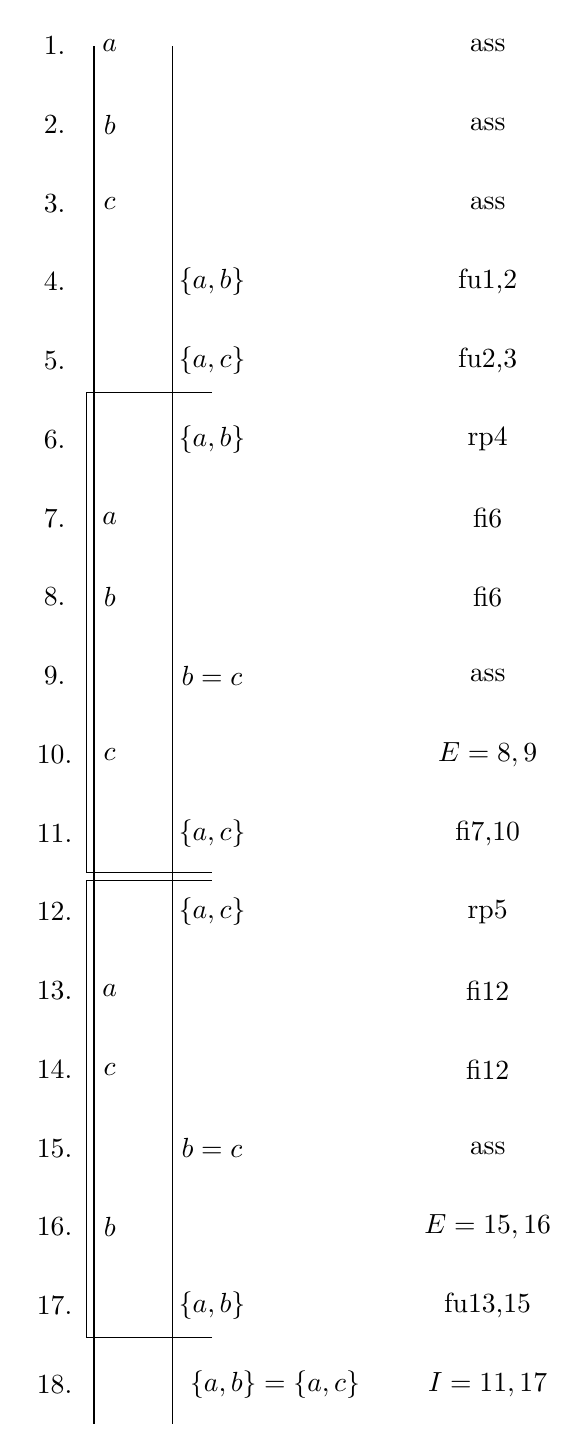
\begin{tikzpicture}
        % Vertical lines
        \draw (0,-9.5) -- (0,8);
        \draw (1,-9.5) -- (1,8);
        \draw (1.5,3.6) -- (-0.1,3.6) -- (-0.1,-2.5) -- (1.5,-2.5);
        \draw (1.5,-8.4) -- (-0.1,-8.4) -- (-0.1,-2.6) -- (1.5,-2.6);
        % Labels between lines
        \node at (-0.5,8) {1.};
        \node at (-0.5,7) {2.};
        \node at (-0.5,6) {3.};
        \node at (-0.5,5) {4.};
        \node at (-0.5,4) {5.};
        \node at (-0.5,3) {6.};
        \node at (-0.5,2) {7.};
        \node at (-0.5,1) {8.};
        \node at (-0.5,0) {9.};
        \node at (-0.5,-1) {10.};
        \node at (-0.5,-2) {11.};
        \node at (-0.5,-3) {12.};
        \node at (-0.5,-4) {13.};
        \node at (-0.5,-5) {14.};
        \node at (-0.5,-6) {15.};
        \node at (-0.5,-7) {16.};
        \node at (-0.5,-8) {17.};
        \node at (-0.5,-9) {18.};
        \node at (0.2,8) {$a$};
        \node at (5,8) {ass};
        \node at (0.2,7) {$b$};
        \node at (5,7) {ass};
        \node at (0.2,6) {$c$};
        \node at (5,6) {ass};
        \node at (1.5,5) {$\{a,b\}$};
        \node at (5,5) {fu1,2};
        \node at (1.5,4) {$\{a,c\}$};
        \node at (5,4) {fu2,3};
        \node at (1.5,3) {$\{a,b\}$};
        \node at (5,3) {rp4};
        \node at (0.2,2) {$a$};
        \node at (5,2) {fi6};
        \node at (0.2,1) {$b$};
        \node at (5,1) {fi6};
        \node at (1.5,0) {$b=c$};
        \node at (5,0) {ass};
        \node at (0.2,-1) {$c$};
        \node at (5,-1) {$E=8,9$};
        \node at (1.5,-2) {$\{a,c\}$};
        \node at (5,-2) {fi7,10};
        \node at (1.5,-3) {$\{a,c\}$};
        \node at (5,-3) {rp5};
        \node at (0.2,-4) {$a$};
        \node at (5,-4) {fi12};
        \node at (0.2,-5) {$c$};
        \node at (5,-5) {fi12};
        \node at (1.5,-6) {$b=c$};
        \node at (5,-6) {ass};
        \node at (0.2,-7) {$b$};
        \node at (5,-7) {$E=15,16$};
        \node at (1.5,-8) {$\{a,b\}$};
        \node at (5,-8) {fu13,15};
        \node at (2.3,-9) {$\{a,b\} = \{a,c\}$};
        \node at (5,-9) {$I=11,17$};
    \end{tikzpicture}

\end{example}

\section{ Membership }

\begin{undefined}
    \textbf{membership} $(\in)$ a binary relation show that an obj is a member of another obj.
\end{undefined}

\begin{Rule}
    \textbf{$I\in$} (this rule is scheme it means it works everywhere for every obj.)

    \begin{tikzpicture}
        % Vertical lines
        \draw (0,0.5) -- (0,4);
        \draw (1,0.5) -- (1,4);
        % \draw (1.5,3.6) -- (-0.1,3.6) -- (-0.1,1.5) -- (1.5,1.5);
        % Labels between lines
        \node at (-0.5,3) {$n.$};
        \node at (-0.5,2) {$m.$};
        \node at (-0.5,1) {$o.$};
        \node at (1.2,3) {$A$};
        \node at (0.2,2) {$a$};
        \node at (3,2) {$fi,n$};
        \node at (1.5,1) {$a \in A$};
        \node at (3,1) {$I\in,n,m$};
    \end{tikzpicture}

    \begin{tikzpicture}
        % Vertical lines
        \draw (0,0.5) -- (0,4);
        \draw (1,0.5) -- (1,4);
        % \draw (1.5,3.6) -- (-0.1,3.6) -- (-0.1,1.5) -- (1.5,1.5);
        % Labels between lines
        \node at (-0.5,3) {$n.$};
        \node at (-0.5,2) {$m.$};
        \node at (-0.5,1) {$o.$};
        \node at (0.2,3) {$a$};
        \node at (1.2,2) {$A$};
        \node at (3,2) {$fu,n$};
        \node at (1.5,1) {$a \in A$};
        \node at (3,1) {$I\in,n,m$};
    \end{tikzpicture}
\end{Rule}

\begin{Rule}
    \textbf{$E\in$}
    (this rule is scheme it means it works everywhere for every obj.)

    \begin{tikzpicture}
        % Vertical lines
        \draw (0,0) -- (0,4);
        \draw (1,0) -- (1,4);
        % \draw (1.5,2.6) -- (-0.1,2.6) -- (-0.1,0.5) -- (1.5,0.5);
        % Labels between lines
        \node at (-0.5,3) {$n.$};
        \node at (-0.5,2) {$m.$};
        \node at (-0.5,1)  {$o.$};
        \node at (1.5,3) {$a \in A$};
        \node at (1.2,2) {$A$};
        \node at (0.2,1) {$a$};
        \node at (3,1) {fiss,$n,m$};
    \end{tikzpicture}

    \begin{tikzpicture}
        % Vertical lines
        \draw (0,0) -- (0,4);
        \draw (1,0) -- (1,4);
        % \draw (1.5,2.6) -- (-0.1,2.6) -- (-0.1,0.5) -- (1.5,0.5);
        % Labels between lines
        \node at (-0.5,3) {$n.$};
        \node at (-0.5,2) {$m.$};
        \node at (-0.5,1) {$o.$};
        \node at (1.5,3) {$a \in A$};
        \node at (0.2,2) {$a$};
        \node at (1.2,1) {$A$};
        \node at (3,1) {fus,$n,m$};
    \end{tikzpicture}
\end{Rule}

\begin{Rule}
    \textbf{$E=$}
    (this rule is scheme it means it works everywhere for every obj.)

    \begin{tikzpicture}
        % Vertical lines
        \draw (0,0) -- (0,4);
        % Labels between lines
        \node at (-0.5,3) {$n.$};
        \node at (-0.5,2) {$m.$};
        \node at (-0.5,1) {$o.$};
        \node at (0.5,3) {$a\in A$};
        \node at (0.5,2) {$a=b$};
        \node at (0.5,1) {$b\in A$};
        \node at (3,1) {$E=$};
    \end{tikzpicture}

    \begin{tikzpicture}
        % Vertical lines
        \draw (0,0) -- (0,4);
        % Labels between lines
        \node at (-0.5,3) {$n.$};
        \node at (-0.5,2) {$m.$};
        \node at (-0.5,1) {$o.$};
        \node at (0.5,3) {$a\in A$};
        \node at (0.55,2) {$A=B$};
        \node at (0.5,1) {$a\in B$};
        \node at (3,1) {$E=$};
    \end{tikzpicture}
\end{Rule}

% \begin{example}
%     \textbf{} $a \in A,a=b /\therefore b \in A$
% \end{example}

% \begin{tikzpicture}
%     % Vertical lines
%     \draw (0,-2.5) -- (0,3);
%     \draw (1,-2.5) -- (1,3);

%     \draw (1.5,2.6) -- (-0.1,2.6) -- (-0.1,-1.5) -- (1.5,-1.5);

%     % Labels between lines
%     \node at (-0.5,3) {1.};
%     \node at (-0.5,2) {2.};
%     \node at (-0.5,1) {3.};
%     \node at (-0.5,0) {4.};
%     \node at (-0.5,-1) {5.};
%     \node at (-0.5,-2) {6.};

%     \node at (1.5,3) {$a \in A$};
%     \node at (1.2,2) {$A$};
%     \node at (3,2) {rpg};
%     \node at (0.2,1) {$a$};
%     \node at (3,1) {$E\in$};
%     \node at (1.5,0) {$a=b$};
%     \node at (0.2,-1) {$b$};
%     \node at (3,-1) {$E=$};
%     \node at (1.5,-2) {$b \in A$};
%     \node at (3,-2) {$I\in$};

% \end{tikzpicture}

\section{Bot}

\begin{undefined}
    \textbf{bot} $(\bot)$ also called "bottom".means impossible, or a logical symbol denoting a
    impossible situation.
\end{undefined}

also called "bottom".means impossible, or a logical symbol denoting a
impossible situation.

\begin{Rule}
    \textbf{$I\bot$} (this rule is scheme it means it works everywhere for every obj.)
    assume that $a_{0} , a_{1} , a_{2} ... a_{n}$ are  distinct obj.if someone says $ a_{0} \in \{a_{1} , a_{2}\}$
    or if someone says $a_{0} = a_{1}$.
    we know it's not right but how do we must show that?
    (see attention 1.1).

    for (rp): \\

    \begin{tikzpicture}
        % Vertical lines
        \draw (0,0) -- (0,4);
        % Labels between lines
        \node at (-0.5,3) {$n.$};
        \node at (-0.5,2) {$m.$};
        \node at (-0.5,1) {$o.$};
        \node at (0.3,3) {$a_{0}$};
        \node at (0.3,2) {$a_{1}$};
        \node at (2,2) {rp1};
        \node at (0.2,1) {$\bot$};
        \node at (2,1) {$I\bot$,$n,m$};
    \end{tikzpicture}
    \\
    for (fu):
    \\

    \begin{tikzpicture}
        % Vertical lines
        \draw (0,0.5) -- (0,4);
        \draw (1,0.5) -- (1,4);
        % \draw (1.5,3.6) -- (-0.1,3.6) -- (-0.1,1.5) -- (1.5,1.5);
        % Labels between lines
        \node at (-0.5,3) {$n.$};
        \node at (-0.5,2) {$m.$};
        \node at (-0.5,1) {$o.$};
        \node at (0.3,3) {$a_{0}$};
        \node at (2,2) {$\{a_{1} , a_{2}... a_{n}\}$};
        \node at (4,2) {fu1};
        \node at (1.2,1) {$\bot$};
        \node at (4,1) {$I\bot$,$n,m$};
    \end{tikzpicture}
    \\
    for (fi):
    \\

    \begin{tikzpicture}
        % Vertical lines
        \draw (0,0.5) -- (0,4);
        \draw (1,0.5) -- (1,4);
        % \draw (1.5,3.6) -- (-0.1,3.6) -- (-0.1,1.5) -- (1.5,1.5);
        % Labels between lines
        \node at (-0.5,3) {$n.$};
        \node at (-0.5,2) {$m.$};
        \node at (-0.5,1) {$o.$};
        \node at (2,3) {$\{a_{1} , a_{2}... a_{n}\}$};
        \node at (0.3,2) {$a_{0}$};
        \node at (4,2) {fi1};
        \node at (1.2,1) {$\bot$};
        \node at (4,1) {$I\bot$,$n,m$};
    \end{tikzpicture}
\end{Rule}

\begin{Rule}
    \textbf{$E\bot$} (this rule is scheme it means it works everywhere for every obj.)
    (see attention 1.1).
    for (rp): \\
    \begin{tikzpicture}
        % Vertical lines
        \draw (0,0) -- (0,4);
        % Labels between lines
        \node at (-0.5,3) {$n.$};
        \node at (-0.5,2) {$m.$};
        \node at (-0.5,1) {$o.$};
        \node at (0.2,3) {$\bot$};
        \node at (0.3,2) {$a_{0}$};
        \node at (0.3,1) {$a_{1}$};
        \node at (4,1) {rp,$n,m$};
    \end{tikzpicture}
    \\
    for (fu):
    \\

    \begin{tikzpicture}
        % Vertical lines
        \draw (0,0) -- (0,3.5);
        \draw (1,0) -- (1,3.5);
        % \draw (1.5,2.6) -- (-0.1,2.6) -- (-0.1,0.5) -- (1.5,0.5);
        % Labels between lines
        \node at (-0.5,3) {$n.$};
        \node at (-0.5,2) {$m.$};
        \node at (-0.5,1) {$o.$};
        \node at (1.2,3) {$\bot$};
        \node at (0.3,2) {$a_{0}$};
        \node at (2,1) {$\{a_{1} , a_{2}... a_{n}\}$};
        \node at (4,1) {fu,$n,m$};
        \\
    \end{tikzpicture}
    \\
    for (fi):
    \\

    \begin{tikzpicture}
        % Vertical lines
        \draw (0,0) -- (0,3.5);
        \draw (1,0) -- (1,3.5);
        % \draw (1.5,2.6) -- (-0.1,2.6) -- (-0.1,0.5) -- (1.5,0.5);
        % Labels between lines
        \node at (-0.5,3) {$n.$};
        \node at (-0.5,2) {$m.$};
        \node at (-0.5,1) {$o.$};
        \node at (1.2,3) {$\bot$};
        \node at (2,2) {$\{a_{1} , a_{2}... a_{n}\}$};
        \node at (0.3,1) {$a_{0}$};
        \node at (4,1) {fiss,$n,m$};
    \end{tikzpicture}

\end{Rule}

% \begin{Rule}
%     \textbf{$I\not=$}
%     (this rule is scheme it means it works everywhere for every obj.)

%     \begin{NiceTabular}{lll}
%         1.     & $a = b$     & acp      \\
%                & $\vdots$    &          \\
%         $n.$   & $\bot$      &          \\
%         $n+1.$ & $a \not= b$ & $I\not=$ \\
%         \CodeAfter \tikz \draw [<-,shorten < = 2pt] (1-1) r-lr (4-|3);
%     \end{NiceTabular}
% \end{Rule}

% \begin{Rule}
%     \textbf{$I\notin$}
%     (this rule is scheme it means it works everywhere for every obj.)

%     \begin{NiceTabular}{lll}
%         1.     & $a \in A$    & acp       \\
%                & $\vdots$     &           \\
%         $n.$   & $\bot$       &           \\
%         $n+1.$ & $a \notin A$ & $I\notin$ \\
%         \CodeAfter \tikz \draw [<-,shorten < = 2pt] (1-1) r-lr (4-|3);
%     \end{NiceTabular}

% \end{Rule}

% \begin{Rule}
%     \textbf{$E\not=$}
%     (this rule is scheme it means it works everywhere for every obj.)

%     \begin{NiceTabular}{lll}
%         $n.$ & $a = b$     &          \\
%         $m.$ & $a \not= b$ &          \\
%         $o.$ & $\bot$      & $E\not=$ \\
%     \end{NiceTabular}
% \end{Rule}

% \begin{Rule}
%     \textbf{$E\notin$}
%     (this rule is scheme it means it works everywhere for every obj.)

%     \begin{NiceTabular}{lll}
%         $n.$ & $a \in A$    &           \\
%         $m.$ & $a \notin A$ &           \\
%         $o.$ & $\bot$       & $E\notin$ \\
%     \end{NiceTabular}

% \end{Rule}

% \begin{Attention}
%     in rules $(I,E)\bot $ obj must be in correct type.for example $\bot$ can't prove
%     $a \in a$.
% \end{Attention}

\section{constants and variables}
obj are two types.we know them and we know what exactly are we talking about
and unknowns are mystery.all the obj we have used until now were known ones we
call them \textbf{"constants"}.

\begin{undefined}
    \textbf{variables} A variable is a symbol
    (usually a letter like $x, y, or z$)
    that represents an unknown obj.
\end{undefined}

\begin{definition}
    \textbf{variables sets} A variable that is a set
    (usually a letter like $X, Y, or Z$)
    that represents an unknown set.
\end{definition}

\begin{definition}
    \textbf{predicate} identity and membership symbols are predicates.
    we will introduce them all to you.
\end{definition}

\chapter{propositional logic(zeroth-order logic)}

\section{What is proposition?}

before answering to this question let me show you what is well formed
formula(WWF).

%
\begin{definition}
    \textbf{Atomic formula} every two obj(conatants and variable) and a binary
    predicate $(=,\in)$ between them like $x=b , y\in C, ...$
    \\
    we denote atomic formulas with $A_{i}$.
\end{definition}

%
\begin{undefined}
    \textbf{logical operators} ($\neg ,\to ,\land ,\lor$) tool that used between
    atoms to make more complex formulas
    (all of the opratores are binary except "$\neg$" that is unary ).
\end{undefined}

%
\begin{definition}
    \textbf{well formed formula(WWF)} these are formulas.

    \begin{enumerate}
        \setlength{\itemsep}{0pt} % No extra space between items
        \item atomic formulas $(A_{i})$
        \item if $A$ is a formula then $\neg A$ is a formula too.
        \item if $A ,B$ are two formulas then $A ** B $ is a formula too.($**$ can be $\to
                  ,\land ,\lor$)
    \end{enumerate}

    for example $(A_0 \to A_1 ,\neg A_3)$ \\ we easily call WWF ``formula'' and
    also we denote WWF with $A ,B ,C ,...$.
\end{definition}

you can easily see that formula are made up by atomic formulas.in general we
say formula is an atomic formula or combination of them.
%
\begin{definition}
    \textbf{open formula} formulas that variables used in one of its atomic formulas.
\end{definition}

the formulas that are not open call \textbf{``closed formulas''} or
\textbf{``sentence''}. Now question is ``are very closed formulas
proposition?'' (propositions in classic logic are sentences that are true or
false?) the answer is unfortunately \textbf{No}.

%
\begin{definition}
    \textbf{Atomic proposition} every atomic formula that can be
    proven by tools introduced in chapter 1($I= , E= , I\in , E\in , I \bot , E\bot $).
    \\
    we denote atomic formulas with $p_{i}$.
\end{definition}

%
\begin{definition}
    \textbf{proposition} every WWF formula that its atomes are all atomic
    propositions.
    \\
    we denote propositions with $p ,q ,r ,...$.
\end{definition}

%
\begin{definition}
    \textbf{Substitution} we define Substitution for a formula like this.
    \begin{enumerate}
        \setlength{\itemsep}{0pt} % No extra space between items
        \item for atomic formulas like $(A_{i})$ if obj was not used before just replace it.
              (example $(a \in A)[b/a]$ is $b \in A$ and if the alternative was in formula.
              it will not change.)
        \item if formula $A$ is complex do it for all atomes.
    \end{enumerate}
\end{definition}

simply means in a formula put an obj like $b$ instead of another like $a$.we
denote it by $A[b/a]$ or $A[\frac{b}{a}]$

\begin{definition}
    \textbf{open proposition} assume formula of a proposition but Substitute some
    obj and replace them with variables.we call it open proposition and denote it with
    capital letter $(P,Q,R)$ showes other types of \textbf{predicates} and variables like$(P(x) ,Q(x,y) ,..)$
\end{definition}

\section{Rules of propositions.}

\begin{definition}
    \textbf{proposition schema(variable proposition)} a proposition that is unknown
    for us and it works as variable.(we show them with $\varphi ,\psi ,\theta ,... $)
\end{definition}

\begin{undefined}
    \textbf{Assumption for conditional proof(acp)} is a tool for assuming a proposition.
    (any proposition can't get out but it can get in. right line must be shoter than left one.(it can't fall out).  and every hypothesis that opens must be closed.)
    % (you will undrestnd what is proposition soon.)

    \begin{fitchproof}[arrayenv=tabular]
        \open
        \have {1} {}
        \open
        \have {2} {}
        \open
        \have {3} {}
        \have {4} {}
        \close
        \have {5} {}
        \close
        \have {6} {}
        \close
    \end{fitchproof}

\end{undefined}

\begin{Rule}
    \textbf{rules of logical operations} $(I\to , E\to ,I\land ,E\land ,I\lor ,E\lor ,I\neg ,E\neg,I\bot ,E\bot )$
    this rule is scheme it means it works everywhere for every propositions.
    (thats why we use $\varphi, \psi $ instead of $p,q$)

    \begin{tabular}{|>{\centering\arraybackslash}m{7cm}|>{\centering\arraybackslash}m{7cm}|}
        \hline
        \begin{fitchproof}[arrayenv=tabular]
            \open
            \have [ ] {1} {\varphi}
            \have [ ] {2} {\vdots}
            \have  [ ] {2} {\psi}
            \close
            \have  [ ]{2} {\therefore \varphi \to \psi} \by{$I\to$}{}
        \end{fitchproof}
         &
        \begin{fitchproof}[arrayenv=tabular]
            \hypo [ ]{1} {\varphi \to \psi}
            \hypo [ ] {2} {\varphi}
            \have  [ ]{2} {\therefore \psi} \by{$E\to$}{}
        \end{fitchproof}
        \\
        \hline
        \begin{fitchproof}[arrayenv=tabular]
            \hypo [ ]{1} {\varphi}
            \hypo [ ] {2} {\psi}
            \have  [ ]{2} {\therefore \varphi \land \psi} \by{$I\land$}{}
        \end{fitchproof}
         &
        \begin{minipage}[t]{\linewidth}
            \centering
            \begin{minipage}[t]{0.48\linewidth}
                \begin{fitchproof}[arrayenv=tabular]
                    \hypo [ ]{1} {\varphi \land \psi}
                    \have [ ]{2} {\therefore \varphi}  \by{$E\land$}{}
                \end{fitchproof}
            \end{minipage}
            % \hfill
            \begin{minipage}[t]{0.48\linewidth}
                \begin{fitchproof}[arrayenv=tabular]
                    \hypo [ ]{1} {\varphi \land \psi}
                    \have [ ]{2} {\therefore\psi} \by{$E\land$}{}
                \end{fitchproof}
            \end{minipage}
        \end{minipage}
        \\
        \hline
        \begin{minipage}[t]{\linewidth}
            \centering
            \begin{minipage}[t]{0.48\linewidth}
        \begin{fitchproof}[arrayenv=tabular]
            \hypo [ ]{1} {\varphi}
            \have  [ ]{2} {\therefore \varphi \lor \psi } \by{$I\lor$}{}
        \end{fitchproof}
            \end{minipage}
            % \hfill
            \begin{minipage}[t]{0.48\linewidth}
        \begin{fitchproof}[arrayenv=tabular]
            \hypo [ ]{1} {\varphi}
            \have  [ ]{2} {\therefore  \psi \lor \varphi} \by{$I\lor$}{}
        \end{fitchproof}
            \end{minipage}
        \end{minipage}

         &
        \begin{fitchproof}[arrayenv=tabular]
            \have [ ] {1} {\varphi \lor \psi}
            \open
            \have [ ] {1} {\varphi}
            \have [ ] {2} {\vdots}
            \have  [ ] {2} {\theta}
            \close
            \open
            \have [ ] {1} {\psi}
            \have [ ] {2} {\vdots}
            \have  [ ] {2} {\theta}
            \close
            \have  [ ]{2} {\therefore \theta} \by{$E\lor$}{}
        \end{fitchproof}
        \\
        \hline
        \begin{fitchproof}[arrayenv=tabular]
            \open
            \have [ ] {1} {\varphi}
            \have [ ] {2} {\vdots}
            \have  [ ] {2} {\bot}
            \close
            \have  [ ]{2} {\therefore \neg\varphi } \by{$I\neg$ }{}
        \end{fitchproof}

         &
        \begin{fitchproof}[arrayenv=tabular]
            \open
            \have [ ] {1} {\neg\varphi}
            \have [ ] {2} {\vdots}
            \have  [ ] {2} {\bot}
            \close
            \have  [ ]{2} {\therefore \varphi } \by{$E\neg$ }{}
        \end{fitchproof}
        \\
        \hline
        \begin{fitchproof}[arrayenv=tabular]
            \hypo [ ]{1} {\varphi}
            \hypo [ ] {2} {\neg\varphi}
            \have  [ ]{2} {\therefore \bot} \by{$I\bot$}{}
        \end{fitchproof}
         &
        \begin{fitchproof}[arrayenv=tabular]
            \hypo [ ] {2} {\bot}
            \have  [ ]{2} {\therefore \varphi} \by{$E\bot$}{}
        \end{fitchproof}
        \\
        \hline
    \end{tabular}

\end{Rule}

\begin{definition}
    \textbf{$\varphi \leftrightarrow \psi$} : $(\varphi \to \psi) \land (\psi \to \varphi)$
\end{definition}

\begin{definition}
    \textbf{schema of prove} you've got knowed by now what is schema of a rule.
    if you want to prove a theorem that it's schema form.you can't prove it directly.
    here we use a technique calls \textbf{"schema of prove"}.
    it let us prove for all situations at the same time.
\end{definition}

\begin{theorem}
    \textbf{$(schema)$} $(I\leftrightarrow , E\leftrightarrow)$

    \begin{tabular}{|>{\centering\arraybackslash}m{7cm}|>{\centering\arraybackslash}m{7cm}|}
        \hline
        \begin{fitchproof}[arrayenv=tabular]
            \open
            \have [ ] {1} {\varphi}
            \have [ ] {2} {\vdots}
            \have  [ ] {2} {\psi}
            \close
            \open
            \have [ ] {1} {\psi}
            \have [ ] {2} {\vdots}
            \have  [ ] {2} {\varphi}
            \close
            \have  [ ]{2} {\therefore \varphi \leftrightarrow \psi} \by{$I\leftrightarrow$}{}
        \end{fitchproof}
         &
        \begin{fitchproof}[arrayenv=tabular]
            \hypo [ ]{1} {\varphi \leftrightarrow \psi}
            \hypo [ ] {2} {\varphi \hspace{0.9cm} \psi}
            \have  [ ]{2} {\therefore \psi \hspace{.5cm} \therefore\varphi} \by{$E\leftrightarrow$}{}
        \end{fitchproof}
        \\
        \hline
    \end{tabular}

    \begin{fitchproof}[arrayenv=tabular]
        \open
        \have  {1} {\varphi}                                            \by{acp  }{}
        \have [ ] {2} {\vdots}
        \have  [n] {2} {\psi}
        \close
        \open
        \have {1} {\psi}                                            \by{acp  }{}
        \have [ ] {2} {\vdots}
        \have  [m] {2} {\varphi}
        \close
        \have   {2} {\varphi \to \psi }                              \by{$I\to,1,n$ }{}
        \have   {2} {\psi \to \varphi }                              \by{$I\to,n+1,m$}{}
        \have  {2} {(\varphi \to \psi)\land (\psi \to \varphi)}     \by{$I\land,m+1,m+2$}{}
        \have  {2} {\varphi \leftrightarrow \psi}                     \by{$Def.,m+3$ }{}
    \end{fitchproof}

    \begin{fitchproof}[arrayenv=tabular]
        \have {1} {\varphi \leftrightarrow \psi }                   \by{ass}{}
        \have {2} {\varphi }                                        \by{ass}{}
        \have  {2} {(\varphi \to \psi)\land (\psi \to \varphi)}     \by{$Def. 1$}{}
        \have  {2} {\varphi \to \psi }                              \by{$E\land 3$}{}
        \have  {2} {\psi}                                           \by{$E\to 1,4$}{}
    \end{fitchproof}

\end{theorem}

\begin{example}
    \textbf{} $a_{0} \notin \{a_{1} , a_{2}... a_{n}\}$

    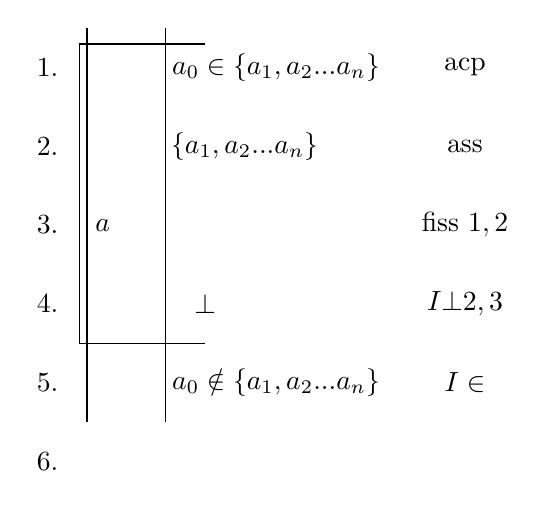
\begin{tikzpicture}
        % Vertical lines
        \draw (0,-1.5) -- (0,3.5);
        \draw (1,-1.5) -- (1,3.5);
        \draw (1.5,3.3) -- (-0.1,3.3) -- (-0.1,-0.5) -- (1.5,-0.5);
        % Labels between lines
        \node at (-0.5,3) {1.};
        \node at (-0.5,2) {2.};
        \node at (-0.5,1) {3.};
        \node at (-0.5,0) {4.};
        \node at (-0.5,-1) {5.};
        \node at (-0.5,-2) {6.};
        \node at (2.4,3) {$a_{0} \in \{a_{1} , a_{2}... a_{n}\}$};
        \node at (4.8,3) {acp};
        \node at (2,2) {$\{a_{1} , a_{2}... a_{n}\}$};
        \node at (4.8,2) {ass};
        \node at (0.2,1) {$a$};
        \node at (4.8,1) {fiss $1,2$};
        \node at (1.5,0) {$\bot$};
        \node at (4.8,0) {$I\bot 2,3$};
        \node at (2.4,-1) {$a_{0} \notin \{a_{1} , a_{2}... a_{n}\}$};
        \node at (4.8,-1) {$I\in$};
    \end{tikzpicture}
\end{example}

\begin{example}
    \textbf{} for conatants p,q,r we can prove these.Proof Is Left As An Exercise To The Reader.\twemoji{1f600}
    \begin{enumerate}
        \setlength{\itemsep}{0pt} % No extra space between items
        \item  $p \rightarrow q, q \rightarrow r /\therefore p \rightarrow r$
        \item  $q /\therefore p \rightarrow q$
        \item $(p \wedge q) \wedge r /\therefore p \wedge(q \wedge r)$
        \item $p \wedge q /\therefore q \wedge p$
        \item $p \rightarrow q /\therefore(p \wedge r) \rightarrow q$
        \item $(p \wedge q) \rightarrow r /\therefore p \rightarrow(q \rightarrow r)$
        \item  $p \rightarrow(q \rightarrow r) /\therefore(p \wedge r) \rightarrow q$
        \item $p \vee q /\therefore q \vee p$
        \item $(p \vee q) \vee r /\therefore p \vee(q \vee r)$
        \item $ p \wedge(q \vee r) /\therefore(p \wedge q) \vee(p \wedge r)$
        \item  $(p \rightarrow q) \wedge(r \rightarrow s) /\therefore(p \vee r) \rightarrow(q \vee s)$
        \item  $p \rightarrow q, \neg q /\therefore \neg p$
        \item  $p \rightarrow q /\therefore \neg p \vee q$

    \end{enumerate}
\end{example}

\begin{exercise}
    \textbf{} for conatants p,q,r prove.
    \begin{enumerate}
        \setlength{\itemsep}{0pt} % No extra space between items
        \item  $p /\therefore p$
        \item  $/\therefore p \vee \neg p$
        \item  $\neg p, p \vee q /\therefore q$
        \item  $\neg p /\therefore p \rightarrow q$
        \item  $p \rightarrow q \therefore /\therefore \neg q \rightarrow \neg p$
        \item  $(p \vee q) \wedge(p \vee r) \therefore /\therefore(p \vee(q \wedge r)) $
        \item  $\neg p \wedge \neg q \therefore /\therefore \neg(p \vee q)$
        \item $\neg p \vee \neg q \therefore /\therefore \neg(p \wedge q)$
        \item  $(\neg p \rightarrow q) /\therefore((p \rightarrow q) \rightarrow q)$
        \item  $/\therefore(p \wedge q \rightarrow r) \wedge(p \wedge s \rightarrow r) \rightarrow(p \wedge(q \vee s) \rightarrow r)$
        \item $/\therefore(p \wedge q \rightarrow r) \vee(p \wedge s \rightarrow r) \rightarrow(p \wedge(q \wedge s) \rightarrow r)$
        \item $/\therefore(p \rightarrow(q \rightarrow r)) \rightarrow((p \rightarrow q) \rightarrow(p \rightarrow r))$
        \item $/\therefore(p \rightarrow q) \rightarrow((q \rightarrow r) \rightarrow(p \rightarrow r))$
    \end{enumerate}
\end{exercise}

\begin{Attention}
    we can rewrite \textbf{Example} and \textbf{Exercise} propositions and
    proofs with proposition schemas and schema of proves.so they are all rules.
\end{Attention}

\chapter{first-order logic}

\section{what is predicate?}

%
\begin{definition}
    \textbf{Big AND and OR} assume a set like $ \{a_{0},a_{1},a_{2},...,a_{n}\}$
    we define \textbf{big AND} like this.
    \\
    \[ \bigwedge\limits_{i=0}^n P(a_{i}) : Pa_{0} \land P(a_{1}) \land P(a_{2}) \land... \land P(a_{n})\]
    \\
    and \textbf{big OR}
    \\
    \[ \bigvee\limits_{i=0}^n P(a_{i}) : P(a_{0}) \lor P(a_{1}) \lor P(a_{2}) \lor... \lor P(a_{n})\]

\end{definition}

\begin{definition}
    \textbf{Universe of discourse} we specify a set like $ \{a_{0},a_{1},a_{2},...,a_{n}\}$
    as universe of a Logic world.

\end{definition}

\begin{Rule}
    \textbf{use of open propositions} assume universe of discourse is $ \{a_{0},a_{1},a_{2},...,a_{n}\}$
    \\
    \begin{fitchproof}[arrayenv=tabular]
        \have [c] {1} {P(x)}
    \end{fitchproof}
    means :
    \\
    \begin{fitchproof}[arrayenv=tabular]
        \have [c_{0}] {1} {P(a_{0})}
        \have [c_{1}] {1} {P(a_{1})}
        \have [c_{2}] {1} {P(a_{2})}
        \have [ ] {2} {\vdots}
        \have [c_{n}] {1} {P(a_{n})}
    \end{fitchproof}
    \par
    if $Px$ was been assemed then like this
    \begin{fitchproof}[arrayenv=tabular]
        \open
        \have [c] {1} {P(x)}
        \have [ ] {2} {\vdots}
        \close
    \end{fitchproof}
    means :
    \begin{fitchproof}[arrayenv=tabular]
        \open
        \have [c_{0}] {1} {P(a_{0})}
        \have [ ] {2} {\vdots}
        \close
        \open
        \have [c_{1}] {1} {P(a_{1})}
        \have [ ] {2} {\vdots}
        \close
        \open
        \have [c_{2}] {1} {P(a_{2})}
        \have [ ] {2} {\vdots}
        \close
        \open
        \have [c_{n}] {1} {P(a_{n})}
        \have [ ] {2} {\vdots}
        \close
    \end{fitchproof}
\end{Rule}
%

\begin{definition}
    \textbf{Universal quantification} assume universe of discourse is $ \{a_{0},a_{1},a_{2},...,a_{n}\}$
    we define $\forall x P(x)$
    \\
    \[ \forall x Px : \bigwedge\limits_{i=0}^n P(a_{i}) \]
\end{definition}

\begin{definition}
    \textbf{Existential quantification} assume universe of discourse is $ \{a_{0},a_{1},a_{2},...,a_{n}\}$
    we define $\exists x Px$
    \\
    \[ \exists  x Px : \bigvee\limits_{i=0}^n P(a_{i}) \]
\end{definition}

\begin{definition}
    \textbf{predicate schema(variable predicate)} a predicate that is unknown
    for us and it works as variable.(we show them with $\Phi ,\Psi ,\Theta ,... $)
\end{definition}

as you can see $\forall x \Phi (x) $ and $\exists x \Phi (x) $ are sentences.

\begin{definition}
    \textbf{Free variables} variables that are not bound by a quantifier.
    (you can easily see that every formula with no free variables are sentences)
    (previously we sayed that every sentece is not necessary a proposition)
\end{definition}

\section{Rules of predicates.}

\begin{theorem}
    \textbf{$(schema)$} $(I\forall ,E\forall ,I\exists , E\exists)$

    \begin{tabular}{|>{\centering\arraybackslash}m{7cm}|>{\centering\arraybackslash}m{7cm}|}
        \hline
        Rules
         &
        Terms and Conditions
        \\
        \hline
        \begin{fitchproof}[arrayenv=tabular]
            \hypo [ ] {2} {\Phi (y)}
            \have  [ ]{2} {\therefore \forall x \Phi (x)} \by{$I\forall$}{}
        \end{fitchproof}
         &
        \begin{enumerate}
            \setlength{\itemsep}{0pt} % No extra space between items
            \item  $y$ is a variable.
            \item  $\Phi (y)$ must not be assumed.
        \end{enumerate}

        \\
        \hline
        \begin{fitchproof}[arrayenv=tabular]
            \hypo [ ] {2} {\forall x \Phi (x)}
            \have  [ ]{2} {\therefore \Phi (a)} \by{$E\forall$}{}
        \end{fitchproof}
         &
        \begin{enumerate}
            \setlength{\itemsep}{0pt} % No extra space between items
            \item  $a$ is an obj in universe of discourse.(it can be constant or variable.)
        \end{enumerate}

        \\
        \hline
        \begin{fitchproof}[arrayenv=tabular]
            \hypo [ ] {2} {\Phi (a)}
            \have  [ ]{2} {\therefore \exists x \Phi (x)} \by{$I\exists$}{}
        \end{fitchproof}

         &

        \begin{enumerate}
            \setlength{\itemsep}{0pt} % No extra space between items
            \item  $a$ is an obj in universe of discourse.(it can be conatant or variable.)
        \end{enumerate}

        \\
        \hline
        \begin{fitchproof}[arrayenv=tabular]
            \have [ ] {1} {\exists x \Phi (x)}
            \open
            \have [ ] {1} {\Phi (y)}
            \have [ ] {2} {\vdots}
            \have  [ ] {2} {\theta}
            \close
            \have  [ ]{2} {\therefore\theta } \by{$E\exists$}{}
        \end{fitchproof}
         &
        \begin{enumerate}
            \setlength{\itemsep}{0pt} % No extra space between items
            \item  $y$ is a variable.
            \item  $\Phi (y)$ must not be assumed in previous lines.(except ones that are closed)
            \item $y$ is not free in $\theta$
        \end{enumerate}
        \\
        \hline
    \end{tabular}
    % \printindex

    \begin{tabular}{>{\centering\arraybackslash}m{7cm}>{\centering\arraybackslash}m{7cm}}
        \begin{fitchproof}[arrayenv=tabular]
            \have  {2} {\Phi (y)}                                         \by{$ass$  }{}
            \have  {2} {\Phi (a_{0})}                                     \by{$Def.1$ }{}
            \have [ ] {2} {\vdots}
            \have [n] {2} {\Phi (a_{n})}                                       \by{$Def.1$}{}
            \have {2} {\bigwedge\limits_{i=0}^n \Phi (a_{i}) }          \by{$I\land,2,3,...,n+2$}{}
            \have  {2} { \forall x \Phi (x)}                  \by{$Def. n+3$ }{}
        \end{fitchproof}
         &
        \begin{fitchproof}[arrayenv=tabular]
            \have  {2} {\forall x \Phi (x)}                         \by{$ass$ }{}
            \have  {2} {\bigwedge\limits_{i=0}^n \Phi (a_{i})}      \by{$Def.1$}{}
            \have  {2} { \Phi (a)}                         \by{$E\land 2$}{}
        \end{fitchproof}

        \\

        \begin{fitchproof}[arrayenv=tabular]
            \have  {2} {\Phi (a)}
            \have  {2} {\bigvee\limits_{i=0}^n \Phi (a_{i})}   \by{$I\lor 1$}{}
            \have  {2} { \exists x \Phi (x)}         \by{$Def 2$}{}
        \end{fitchproof}

         &

        \begin{fitchproof}[arrayenv=tabular]
            \have  {1} {\exists x \Phi (x)}
            \have  {1} {\bigvee\limits_{i=0}^n \Phi (a_{i}) }
            \open
            \have  {1} {\Phi (a_{0})}                  \by{acp  }{}
            \have [ ] {2} {\vdots}
            \have  [n] {2} {\theta}
            \close
            \open
            \have  {1} {\Phi (a_{1})}                \by{acp  }{}
            \have [ ] {2} {\vdots}
            \have  [m] {2} {\theta}
            \close
            \have [ ] {2} {\vdots}
            \open
            \have [l] {1} {\Phi (a_{2})}                    \by{acp  }{}
            \have [ ] {2} {\vdots}
            \have  [r] {2} {\theta}
            \close
            \have  {2} {\theta }                    \by{$E\exists$}{}
        \end{fitchproof}

    \end{tabular}

\end{theorem}

\begin{example}
    \textbf{}for conatants P,Q,R we can prove these.Proof Is Left As An Exercise To The Reader.\twemoji{1f600}

    \begin{enumerate}
        \setlength{\itemsep}{0pt} % No extra space between items

        \item   $ \forall x(P(x) \wedge Q(x)) \therefore / \therefore \forall x P(x) \wedge \forall x Q(x) $
        \item   $ \exists x(P(x) \vee Q(x)) \therefore /\therefore \exists x P(x) \vee \exists x Q(x) $
        \item   $ \forall x P(x) \vee \forall x Q(x) /\therefore \forall x(P(x) \vee Q(x)) $
        \item   $ \exists x(P(x) \wedge Q(x)) /\therefore \exists x P(x) \wedge \exists x Q(x) $
        \item   $ \forall x(P(x) \rightarrow Q(x)) /\therefore  \forall x P(x) \rightarrow \forall x Q(x) $
        \item   $\exists x P(x) \rightarrow \exists x Q(x) /\therefore \exists x(P(x) \rightarrow Q(x)) $
        \item   $ \forall x P(x) \wedge Q \therefore /\therefore \forall x(P(x) \wedge Q) $
        \item   $ \forall x P(x) \vee Q \therefore /\therefore \forall x(P(x) \vee Q) $
        \item   $ \exists x P(x) \wedge Q \therefore /\therefore \exists x(P(x) \wedge Q) $
        \item   $ \exists x P(x) \vee Q \therefore /\therefore \exists x(P(x) \vee Q) $
        \item   $Q \rightarrow \forall x P(x) \therefore /\therefore \forall x(Q \rightarrow P(x)) $
        \item   $Q \rightarrow \exists x P(x) \therefore /\therefore \exists x(Q \rightarrow P(x)) $
        \item   $\forall x P(x) \rightarrow Q \therefore /\therefore \exists x(P(x) \rightarrow Q) $
        \item   $\exists x P(x) \rightarrow Q \therefore /\therefore \forall x(P(x) \rightarrow Q) $
        \item   $ \exists x \neg P(x) \therefore /\therefore \neg \forall x P(x)  $
        \item   $ \forall x \neg P(x) \therefore /\therefore \neg \exists x P(x) $

    \end{enumerate}
\end{example}

\begin{exercise}
    \textbf{}for conatants P,Q,R prove.
    \begin{enumerate}
        \setlength{\itemsep}{0pt} % No extra space between items
        \item   $ \exists x \Big(P(x) \wedge \exists y Q(y) \rightarrow \forall z R(z)\Big) /\therefore \forall y \forall z \Big(\forall x P(x) \wedge Q(y) \rightarrow R(z)\Big) $
        \item   $ \forall x \exists y \Big(P(x) \wedge Q(y) \rightarrow \forall z R(z)\Big) /\therefore \forall z \Big(\exists x P(x) \wedge \forall y Q(y) \rightarrow R(z)\Big) $
        \item   $\forall x P(x) \rightarrow \exists y Q(y) /\therefore \exists x \exists y \Big(P(x) \rightarrow Q(y)\Big) $
        \item   $ \forall x \forall z \exists y \exists w \Big(P(y,z) \vee Q(z) \rightarrow R(x,w)\Big) /\therefore \Big(\exists z \forall y P(y,z) \vee \exists z Q(z)\Big) \rightarrow \forall x \exists w R(x,w) $
        \item   $ \exists x P(x) \vee \exists x \Big(Q(x) \wedge R(x) \Big) /\therefore \exists x \Big(P(x) \vee Q(x) \Big) \wedge \exists x \Big(P(x) \vee R(x)\Big) $
        \item   $\exists x \exists z \forall y \Big(P(x,y) \rightarrow Q(z) \vee R(x,y) \Big) /\therefore \forall x \exists y P(x,y) \rightarrow \Big(\exists z Q(z) \vee \exists x \exists z R(x,y)\Big) $
        \item   $ \forall x \exists y \Big(\exists z P(x,y,z) \wedge Q(x,y)\Big) \vee \forall x \exists y \exists z \Big(P(x,y,z) \wedge R(x,y)\Big) /\therefore \forall x \exists y \exists z \Big(P(x,y,z) \wedge(Q(x,y) \vee R(x,y))\Big) $
    \end{enumerate}
\end{exercise}

\begin{Attention}
    we can rewrite \textbf{Example} and \textbf{Exercise} propositions and
    proofs with proposition schemas and schema of proves.so they are all rules.
\end{Attention}

\chapter{The beginning of set theory}

\section{Axioms of set theory}
we emphasis before that set has no definition.but we can describe what set is
with rules and axioms.

\begin{axiom}
    \textbf{Existence of universe of set theory}
    There exists a set $V$ (we denote it as V.it simply means the set of all sets), known as the Von Neumann Universe, which contains every set.
    (this axiom can't be formolized in first order logic).
    (there must be another axiom let us use logic for set theory but we ignore that)
\end{axiom}

\begin{definition}
    \textbf{Subset} a subset is a set where every element is also an element of another, larger set called the superset
    \[ A \subseteq B: \forall x(x \in A \rightarrow x \in B) \]
\end{definition}

\begin{theorem}
    \textbf{$(schema)$} $(I\subseteq , E\subseteq)$

    \begin{tabular}{|>{\centering\arraybackslash}m{7cm}|>{\centering\arraybackslash}m{7cm}|}
        \hline
        \begin{fitchproof}[arrayenv=tabular]
            \open
            \have [ ] {1} {x \in A}
            \have [ ] {2} {\vdots}
            \have  [ ] {2} {x \in B}
            \close
            \have  [ ]{2} {\therefore A \subseteq B  } \by{$I\subseteq$}{}
        \end{fitchproof}

         &
        \begin{fitchproof}[arrayenv=tabular]
            \hypo [ ]{1} {A \subseteq B}
            \hypo [ ] {2} {a \in A}
            \have  [ ]{2} {\therefore  a \in B} \by{$E\subseteq$}{}
        \end{fitchproof}
        \\
        \hline
    \end{tabular}

    \begin{tabular}{>{\centering\arraybackslash}m{7cm}>{\centering\arraybackslash}m{7cm}}
        \begin{fitchproof}[arrayenv=tabular]
            \open
            \have {1} {x \in A}                                         \by{acp}{}
            \have [ ] {2} {\vdots}
            \have  [n] {2} {x \in B}
            \close
            \have  {2} {x \in A \rightarrow x \in B }              \by{$I\rightarrow,1,n$ }{}
            \have  {2} {\forall x(x \in A \rightarrow x \in B )}   \by{$I\forall,n+1$ }{}
            \have  {2} {A \subseteq B  }                           \by{$Def.n+2$ }{}
        \end{fitchproof}
         &
        \begin{fitchproof}[arrayenv=tabular]
            \have {1} {A \subseteq B}                               \by{ass }{}
            \have  {2} {a \in A}                                   \by{ass }{}
            \have  {2} {\forall x(x \in A \rightarrow x \in A )}   \by{$Def.1$ }{}
            \have  {2} {a \in A \rightarrow a \in B }             \by{$E\forall,4$ }{}
            \have  {2} {  a \in B}                                   \by{$E\rightarrow 3,5$}{}
        \end{fitchproof}
        \\
    \end{tabular}

\end{theorem}

\begin{example}
    \textbf{} $A \subseteq B , B \subseteq C/\therefore A \subseteq C$
    \begin{fitchproof}[arrayenv=tabular]
        \have{1} {A \subseteq B }                 \by{ass}{}
        \have {2} {B \subseteq C}                  \by{ass}{}
        \open
        \have   {2} {x \in A }                     \by{$acp$}{}
        \have   {2} {x \in B }                     \by{$E\subseteq ,1,3$ }{}
        \have {1} {x \in C  }                       \by{$E\subseteq ,2,4$}{}
        \close
        \have  {2} {A \subseteq C }             \by{$I\subseteq ,3,5$}{}
    \end{fitchproof}
\end{example}

\begin{axiom}
    \textbf{Extensionality}Two sets are equal (are the same set) if they have the same elements.
    \\
    \[  \forall X,Y (\forall x ( x \in X \leftrightarrow x \in Y ) \rightarrow X = Y )  \]
\end{axiom}

so we can rewrite axiom of Extensionality like this.

\[ \forall X,Y ((X \subseteq Y \wedge Y \subseteq X) \rightarrow X=Y)\]

\begin{theorem}
    \textbf{$(schema)$} $(I= , E=)$

    \begin{tabular}{|>{\centering\arraybackslash}m{7cm}|>{\centering\arraybackslash}m{7cm}|}
        \hline
        \begin{fitchproof}[arrayenv=tabular]
            \open
            \have [ ] {1} {x \in A }
            \have [ ] {2} {\vdots}
            \have  [ ] {2} {x \in B}
            \close
            \open
            \have [ ] {1} {x \in B}
            \have [ ] {2} {\vdots}
            \have  [ ] {2} {x \in A}
            \close
            \have  [ ]{2} {\therefore A = B } \by{$I=$}{}
        \end{fitchproof}
         &
        \begin{fitchproof}[arrayenv=tabular]
            \hypo [ ]{1} {A = B }
            \hypo [ ] {2} {a \in A \hspace{0.9cm} a \in B}
            \have  [ ]{2} {\therefore  a \in B \hspace{.5cm} \therefore  a \in A} \by{$E=$}{}
        \end{fitchproof}
        \\
        \hline
    \end{tabular}

    \begin{fitchproof}[arrayenv=tabular]
        \open
        \have  {1} {x \in A }                                                                 \by{acp  }{}
        \have [ ] {2} {\vdots}
        \have  [n] {2} {x \in B}
        \close
        \have   {2} {A \subseteq B }                                                        \by{$I\subseteq,1,n$  }{}
        \open
        \have  {1} {x \in B}                                                                \by{acp }{}
        \have [ ] {2} {\vdots}
        \have  [m] {2} {x \in A}
        \close
        \have  {2} {B \subseteq A }                                                          \by{$I\subseteq,n+2,m$ }{}
        \have  {2} {\forall X, Y((X \subseteq Y \wedge Y \subseteq X) \rightarrow X=Y)}   \by{Extensionality }{}
        \have  {2} {(A \subseteq B \wedge B \subseteq A) \rightarrow A=B}                 \by{$E\forall,m+2$ }{}
        \have  {2} {A \subseteq B \wedge B \subseteq A}                                       \by{$I\wedge,n+1,m+1$}{}
        \have  {2} {A=B}                                                                        \by{$E\rightarrow,m+3,m+4$}{}
    \end{fitchproof}
    \par
    % \begin{fitchproof}[arrayenv=tabular]
    %     \have {1} {A = B }
    %     \have  {2} {a \in A }
    %     \have  {2} {\forall X, Y((X \subseteq Y \wedge Y \subseteq X) \leftrightarrow X=Y)}    \by{Extensionality}{}
    %     \have  {2} {(A \subseteq B \wedge B \subseteq A) \leftrightarrow A=B}                   \by{$E\forall,3$ }{}
    %     \have  {2} {A \subseteq B \wedge B \subseteq A}                                          \by{$E\leftrightarrow,1,4$}{}
    %     \have  {2} {A \subseteq B}                                                              \by{$E\wedge 5$}{}
    %     \have  {2} {  a \in B }                                                                   \by{$E\subseteq,2,6$ }{}
    % \end{fitchproof}
\end{theorem}

\begin{axiom}
    \textbf{Weak comprehension} this axioms says for every open proposition with just one variable
    like $\Phi(x)$ there is a set such that every $x$ is a member of that set if and only if it holds
    $\Phi(x)$.
    \\
    \[ \exists X \forall x  (\Phi (x) \leftrightarrow x \in X) \]
    \\
    by axiom of extentionality we can show that y is unique.
    so we denote it as $\{ x | \Phi (x)\}$.
\end{axiom}

this axiom show that why Russell's paradox doesn't happened here because if ou
assume $R=\{x|x \notin x\}$ is a set.you can't prove or disprove $R \in R$. (we
don't need to prove that now.we will prove it in \textbf{'MetaLogic'}.)

\section{Definitions of set theory}
Let's talk about some definitions in set theoty.These definitions will come in
handy later.

\begin{definition}
    \textbf{Empty set} also known as the null set,
    is the unique mathematical set containing no elements at all.
    (uniqueness can be proven.)
    \[ \emptyset:=\{x \mid \perp\} \]
    therefore.
    \[ \forall x(x \in \emptyset \leftrightarrow  \perp) \]
    therefore.
    \[ \forall x(x \notin \emptyset ) \]
\end{definition}

\begin{example}
    \textbf{} $/\therefore \forall X(\emptyset \subseteq X)$
    \begin{fitchproof}[arrayenv=tabular]
        \open
        \have{1} {x \in \emptyset}                                \by{acp}{}
        \have {2} {\forall x(x \notin \emptyset)}                  \by{lemma $4.4.1 $ }{}
        \have   {2} {x \notin \emptyset}                           \by{$E\forall ,2$}{}
        \have   {2} {\bot}                                          \by{$I\bot ,1,3$ }{}
        \have {1} {x \in X  }                                        \by{$E\bot ,4$}{}
        \close
        \have  {2} {\emptyset \subseteq X}                       \by{$I\subseteq ,1,5$}{}
        \have  {2} {\forall X(\emptyset \subseteq X)}             \by{$I\forall ,6$}{}
    \end{fitchproof}
\end{example}

\begin{lemma}
    \textbf{} $A = \emptyset \therefore / \therefore \forall y( y \notin A)$
    \begin{fitchproof}[arrayenv=tabular]
        \have  {1} {\forall y (y \notin A )}                                \by{ass}{}
        \open
        \have  {1} {y \in A }                                               \by{acp}{}
        \have  {1} {y \notin A }                                            \by{$E\forall,1$}{}
        \have  {2} {\bot}                                                  \by{$I\bot,2,3$}{}
        \have   {2} {y \in \emptyset }                                       \by{$E\bot,4$ }{}
        \close
        \open
        \have   {2} {y \in \emptyset }                                      \by{acp}{}
        \have  {1} {\forall y (y \notin \emptyset  )}                        \by{Def.}{}
        \have {2} {y \notin \emptyset  }                                    \by{$E\forall,7$  }{}
        \have   {2} {\bot}                                                 \by{$I\bot,6,8$ }{}
        \have   {2} {y \in A}                                                 \by{$E\bot,9$}{}
        \close
        \have  {2} {A = \emptyset }                                                    \by{$I=$}{}
    \end{fitchproof}

    \begin{fitchproof}[arrayenv=tabular]
        \have  {2} {A = \emptyset }                                                    \by{ass}{}
        \open
        \have  {1} {y \in A }                                               \by{acp}{}
        \have  {1} {\forall y (y \notin \emptyset )}                                \by{Def.}{}
        \have   {2} {y \in \emptyset }                                       \by{$E=,1,2$}{}
        \have   {2} {y \notin \emptyset }                                    \by{$E\forall,3$ }{}
        \have  {2} {\bot}                                                  \by{$I\bot,4,5$ }{}
        \close
        \have  {1} {y \notin A }                                            \by{$I\neg$}{}
        \have  {1} {\forall y (y \notin A )}                                \by{$I\forall,7$}{}
    \end{fitchproof}
\end{lemma}

\begin{theorem}
    \textbf{$(schema)$} $(I\emptyset\not= , E \emptyset \not= ,I\emptyset= , E\emptyset=)$

    \begin{tabular}{|>{\centering\arraybackslash}m{7cm}|>{\centering\arraybackslash}m{7cm}|}
        \hline
        \begin{fitchproof}[arrayenv=tabular]
            \hypo [ ] {2} {a \in A}
            \have  [ ]{2} {\therefore A \not= \emptyset} \by{$I\emptyset\not=$}{}
        \end{fitchproof}
         &
        \begin{fitchproof}[arrayenv=tabular]
            \have [ ] {1} {A \not= \emptyset }
            \open
            \have [ ] {1} {x \in A}
            \have [ ] {2} {\vdots}
            \have  [ ] {2} {\theta}
            \close
            \have  [ ]{2} {\therefore\theta } \by{$E \emptyset \not=$}{}
        \end{fitchproof}
        \\
        \hline
        \begin{fitchproof}[arrayenv=tabular]
            \open
            \have [ ] {1} {x \in A}
            \have [ ] {2} {\vdots}
            \have  [ ] {2} {\bot }
            \close
            \have  [ ]{2} {\therefore A = \emptyset } \by{$I\emptyset=$}{}
        \end{fitchproof}
         &
        \begin{fitchproof}[arrayenv=tabular]
            \hypo [ ] {2} {A = \emptyset }
            \have  [ ]{2} {\therefore a \notin A} \by{$E\emptyset=$}{}
        \end{fitchproof}
        \\
        \hline
    \end{tabular}

    \begin{tabular}{>{\centering\arraybackslash}m{7cm}>{\centering\arraybackslash}m{7cm}}
        \begin{fitchproof}[arrayenv=tabular]
            \have  {2} {a \in A}                         \by{ass}{}
            \have  {2} {\exists x(x \in A)}             \by{$I\exists,1$ }{}
            \have  {2} {\neg (\forall x(x \notin A))}   \by{De Morgan $2$ }{}
            \have  {2} { A \not= \emptyset}             \by{lemma $4.4.1 , 3$}{}
        \end{fitchproof}

         &
        \begin{fitchproof}[arrayenv=tabular]
            \have {1} {A \not= \emptyset }              \by{ass}{}
            \have  {2} {\neg (\forall x(x \notin A))}   \by{lemma $4.4.1 , 3$}{}
            \have  {2} {\exists x(x \in A)}             \by{De Morgan $2$ }{}
            \open
            \have{1} {x \in A}                           \by{acp}{}
            \have [ ] {2} {\vdots}
            \have  [n] {2} {\theta}
            \close
            \have  [n+1]{2} {\theta }                    \by{$E\exists$}{}
        \end{fitchproof}
        \\
        \begin{fitchproof}[arrayenv=tabular]
            \open
            \have{1} {x \in A}                           \by{acp}{}
            \have [ ] {2} {\vdots}
            \have  [n] {2} {\bot}
            \close
            \have {1} {x \notin A  }             \by{$I\neg $ }{}
            \have  {2} {\forall x(x \notin A)}   \by{$I\forall ,n+1$}{}
            \have  {2} {A = \emptyset }             \by{lemma $4.4.1 , 1$}{}
        \end{fitchproof}

         &
        \begin{fitchproof}[arrayenv=tabular]
            \have  {2} { A = \emptyset}             \by{ass}{}
            \have  {2} {\forall x(x \notin A)}   \by{lemma $4.4.1 , 1$}{}
            \have  {2} {a \notin A}               \by{$E\forall 2$  }{}
        \end{fitchproof}
        \\

    \end{tabular}
\end{theorem}

\begin{definition}
    \textbf{pairing set}
    \[ \{a_{0}, a_{1}, a_{2}, ... ,a_{n} \}:=\{x \mid x=a_{0} \lor x=a_{1} \lor x=a_{2} \lor ... \lor x=a_{n} \} \]
    therefore.
    \[\forall x( x \in \{a_{0}, a_{1}, a_{2}, ... ,a_{n} \} \leftrightarrow  (x=a_{0} \lor x=a_{1} \lor x=a_{2} \lor ... \lor x=a_{n} )) \]
\end{definition}

\begin{theorem}
    \textbf{$(schema)$} $(I\{\} , E\{\})$

    \begin{tabular}{|>{\centering\arraybackslash}m{7cm}|>{\centering\arraybackslash}m{7cm}|}
        \hline
        \begin{fitchproof}[arrayenv=tabular]
            \hypo [ ] {2} {a = a_{i} }
            \have  [ ]{2} {\therefore  a \in  \{a_{0}, a_{1}, a_{2}, ... ,a_{n} \}} \by{$I\{\}$}{}
        \end{fitchproof}
         &
        \begin{fitchproof}[arrayenv=tabular]
            \have [ ] {1} {a \in  \{a_{0}, a_{1}, a_{2}, ... ,a_{n} \} }
            \open
            \have [ ] {1} {a = a_{0} }
            \have [ ] {2} {\vdots}
            \have  [ ] {2} {\theta}
            \close
            \have [ ] {2} {\vdots}
            \open
            \have [ ] {1} {a = a_{n}}
            \have [ ] {2} {\vdots}
            \have  [ ] {2} {\theta}
            \close
            \have  [ ]{2} {\therefore\theta } \by{$E\{\}$}{}
        \end{fitchproof}
        \\
        \hline
    \end{tabular}
    \\
    \\
    \\
    Proof Is Left As An Exercise To The Reader.\twemoji{1f600}
\end{theorem}

\begin{definition}
    \textbf{Union and Intersection} \\
    Intersection:
    \[ A \cap B:=\{x \mid x \in A \wedge x \in B \} \]
    therefore.
    \[\forall x( x \in A \cap B  \leftrightarrow  (x \in A \wedge x \in B )) \]
    Union:
    \[ A \cup B:=\{x \mid x \in A \lor x \in B \} \]
    therefore.
    \[\forall x( x \in A \cup B  \leftrightarrow  (x \in A \lor x \in B )) \]
\end{definition}

\begin{theorem}
    \textbf{$(schema)$} $(I\cap , E\cap , I\cup , E\cup)$

    \begin{tabular}{|>{\centering\arraybackslash}m{7cm}|>{\centering\arraybackslash}m{7cm}|}
        \hline
        \begin{fitchproof}[arrayenv=tabular]
            \hypo [ ] {2} {a \in A}
            \hypo [ ] {2} {a \in B  }
            \have  [ ]{2} {\therefore  a \in  A \cap B } \by{$I\cap$}{}
        \end{fitchproof}
         &
        \begin{fitchproof}[arrayenv=tabular]
            \hypo [ ] {2} {a \in  A \cap B }
            \have  [ ]{2} {\therefore a \in  A \hspace{.5cm}  \therefore  a \in  B } \by{$E\cap$}{}
        \end{fitchproof}
        \\
        \hline
        \begin{fitchproof}[arrayenv=tabular]
            \hypo [ ] {2} {a \in A   }
            \have  [ ]{2} {\therefore   a \in  A \cup B \hspace{.5cm}  \therefore  a \in  B \cup A } \by{$I\cup$}{}
        \end{fitchproof}
         &
        \begin{fitchproof}[arrayenv=tabular]
            \have [ ] {1} { a \in  A \cup B  }
            \open
            \have [ ] {1} {a \in A }
            \have [ ] {2} {\vdots}
            \have  [ ] {2} {\theta}
            \close
            \open
            \have [ ] {1} { a \in B }
            \have [ ] {2} {\vdots}
            \have  [ ] {2} {\theta}
            \close
            \have  [ ]{2} {\therefore\theta } \by{$E\cup$}{}
        \end{fitchproof}
        \\
        \hline
    \end{tabular}
    \\
    \\
    \\
    Proof Is Left As An Exercise To The Reader.\twemoji{1f600}
\end{theorem}

\begin{definition}
    \textbf{Big Union and Intersection} \\
    Intersection:
    \[  \bigcap A:=\{x \mid \forall X (X \in A \rightarrow x \in X) \} \]
    therefore.
    \[\forall x \Big( x \in \bigcap A  \leftrightarrow  \forall X (X \in A \rightarrow x \in X)\Big) \]
    Union:
    \[  \bigcup A:=\{x \mid \exists X (X \in A \wedge x \in X) \} \]
    therefore.
    \[\forall x( x \in \bigcup A \leftrightarrow  (\exists X (X \in A \wedge x \in X))) \]
\end{definition}

\begin{theorem}
    \textbf{$(schema)$} $(I\bigcap , E\bigcap , I\bigcup , E\bigcup)$

    \begin{tabular}{|>{\centering\arraybackslash}m{7cm}|>{\centering\arraybackslash}m{7cm}|}
        \hline
        \begin{fitchproof}[arrayenv=tabular]
            \open
            \have [ ] {1} {X \in A }
            \have [ ] {2} {\vdots}
            \have  [ ] {2} {a \in X}
            \close
            \have  [ ]{2} {\therefore a \in \bigcap A } \by{$I\bigcap$}{}
        \end{fitchproof}
         &
        \begin{fitchproof}[arrayenv=tabular]
            \hypo [ ] {2} {a \in \bigcap A }
            \hypo [ ] {2} {B \in  A  }
            \have  [ ]{2} {\therefore  a \in  B} \by{$E\bigcap$}{}
        \end{fitchproof}
        \\
        \hline
        \begin{fitchproof}[arrayenv=tabular]
            \hypo [ ] {2} {a \in B  }
            \hypo [ ] {2} {B \in A  }
            \have  [ ]{2} {\therefore  a \in \bigcup A } \by{$I\bigcup$}{}
        \end{fitchproof}
         &
        \begin{fitchproof}[arrayenv=tabular]
            \have [ ] {1} { a \in \bigcup A  }
            \open
            \have [ ] {1} {a \in X \wedge X \in A }
            \have [ ] {2} {\vdots}
            \have  [ ] {2} {\theta}
            \close
            \have  [ ]{2} {\therefore\theta } \by{$E\bigcup$}{}
        \end{fitchproof}
        \\
        \hline
    \end{tabular}
    \\
    \\
    \\
    Proof Is Left As An Exercise To The Reader.\twemoji{1f600}
\end{theorem}

\begin{definition}
    \textbf{Complement}
    \[   A^c:=\{x \mid x \notin A  \} \]
    therefore.
    \[\forall x( x \in A^c \leftrightarrow  x \notin A ) \]
\end{definition}

\begin{theorem}
    \textbf{$(schema)$} $(I()^c, E()^c)$

    \begin{tabular}{|>{\centering\arraybackslash}m{7cm}|>{\centering\arraybackslash}m{7cm}|}
        \hline
        \begin{fitchproof}[arrayenv=tabular]
            \open
            \have [ ] {1} {a \in  A }
            \have [ ] {2} {\vdots}
            \have  [ ] {2} {\bot}
            \close
            \have  [ ]{2} {\therefore a \notin  A} \by{$I()^c$}{}
        \end{fitchproof}
         &
        \begin{fitchproof}[arrayenv=tabular]
            \open
            \have [ ] {1} {a \notin  A }
            \have [ ] {2} {\vdots}
            \have  [ ] {2} {\bot}
            \close
            \have  [ ]{2} {\therefore a \in  A} \by{$E()^c$}{}
        \end{fitchproof}
        \\
        \hline
    \end{tabular}
    \\
    \\
    \\
    Proof Is Left As An Exercise To The Reader.\twemoji{1f600}
\end{theorem}

\begin{observation}
    \textbf{}we can show Universal set with...
    \[   V=\{x \mid \top \} \]
    therefore.
    \[\forall x( x \in V \leftrightarrow  \top ) \]
    therefore.
    \[\forall x( x \in V ) \]
\end{observation}

\begin{definition}
    \textbf{Subtraction}
    \[ A - B:=\{x \mid x \in A \wedge x \notin B \} \]
    therefore.
    \[\forall x \Big( x \in A - B  \leftrightarrow  (x \in A \wedge x \notin B ) \Big) \]
\end{definition}

\begin{theorem}
    \textbf{$(schema)$} $(I- , E- )$

    \begin{tabular}{|>{\centering\arraybackslash}m{7cm}|>{\centering\arraybackslash}m{7cm}|}
        \hline
        \begin{fitchproof}[arrayenv=tabular]
            \hypo [ ] {2} {a \in A  }
            \hypo [ ] {2} {a \notin B  }
            \have  [ ]{2} {\therefore  a \in A - B } \by{$I-$}{}
        \end{fitchproof}
         &
        \begin{fitchproof}[arrayenv=tabular]
            \hypo [ ] {2} {a \in  A - B  }
            \have  [ ]{2} {\therefore  a \in  A \hspace{.5cm}  \therefore  a \notin  B  } \by{$E-$}{}
        \end{fitchproof}
        \\
        \hline
    \end{tabular}
    \\
    \\
    \\
    Proof Is Left As An Exercise To The Reader.\twemoji{1f600}
\end{theorem}

\begin{lemma}
    \textbf{} $/ \therefore  A - B = A \cap B^c$
    \\
    \\
    Proof Is Left As An Exercise To The Reader.\twemoji{1f600}
\end{lemma}

\begin{definition}
    \textbf{Powerset}
    \[ P(A):=\{X \mid X \subseteq A \} \]
    therefore.
    \[\forall X \Big( X \in P(A) \leftrightarrow  (X \subseteq A )\Big) \]
\end{definition}

\begin{theorem}
    \textbf{$(schema)$} $(IP, EP )$

    \begin{tabular}{|>{\centering\arraybackslash}m{7cm}|>{\centering\arraybackslash}m{7cm}|}
        \hline
        \begin{fitchproof}[arrayenv=tabular]
            \hypo [ ] {2} {A \subseteq B }
            \have  [ ]{2} {\therefore   A \in  P(B) } \by{$IP$}{}
        \end{fitchproof}
         &
        \begin{fitchproof}[arrayenv=tabular]
            \hypo [ ] {2} {A \in  P(B) }
            \have  [ ]{2} {\therefore  A \subseteq B } \by{$EP$}{}
        \end{fitchproof}
        \\
        \hline
    \end{tabular}
    \\
    \\
    \\
    Proof Is Left As An Exercise To The Reader.\twemoji{1f600}
\end{theorem}

\chapter{Relations and functions}

\section{cartesian product}

\begin{definition}
    \textbf{Ordered pair}
    \[ (x,y) := \{ \{x\},\{x,y\} \}. \]
\end{definition}

\begin{definition}
    \textbf{Tuples}(n is a arbitrary number.)(this is a temporary definition, we will give a better one in the next chapter.)
    \[ (x_1,x_2,...,x_n) := ((x_1,x_2,...,x_{n-1}),x_n) \]
\end{definition}

\begin{lemma}
    \textbf{} $/ \therefore  (x_0,y_0) = (x_1,y_1) \leftrightarrow ((x_0=x_1) \wedge (y_0=y_1))$
    \\
    \\
    Proof Is Left As An Exercise To The Reader.\twemoji{1f600}
\end{lemma}

\begin{definition}
    \textbf{Cartesian product}
    \[ A \times B := \{ u \mid \exists x,y \Big((x,y)=u \land x \in A \land y\in B \Big)\}. \]
    or i.e.
    \[ A \times B := \{ (x,y) \mid x \in A \land y\in B \}. \]
\end{definition}

\begin{example}
    if
    $ A= \{ a,b,c \}$
    and
    $ B= \{ 0,1,2,3 \} $
    then
    \[ A \times B = \{ (a,0),(a,1),(a,2),(a,3),(b,0),(b,1),(b,2),(b,3),(c,0),(c,1),(c,2),(c,3) \} \]

    %\tikzset{every picture/.style={line width=0.75pt}} %set default line width to 0.75pt        
    \begin{center}
        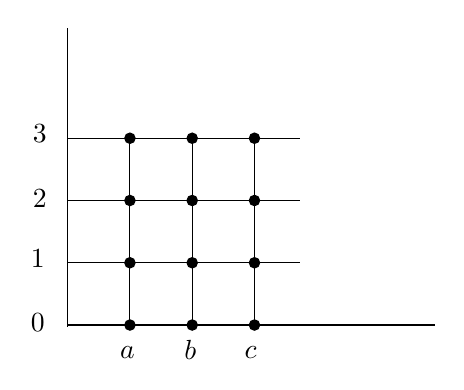
\begin{tikzpicture}[x=0.75pt,y=0.75pt,yscale=-1,xscale=1]
            %uncomment if require: \path (0,236); %set diagram left start at 0, and has height of 236

            %Shape: Grid [id:dp8962445968853252] 
            \draw  [draw opacity=0] (238,106.71) -- (350,106.71) -- (350,197.71) -- (238,197.71) -- cycle ; \draw   (238,106.71) -- (238,197.71)(268,106.71) -- (268,197.71)(298,106.71) -- (298,197.71)(328,106.71) -- (328,197.71) ; \draw   (238,106.71) -- (350,106.71)(238,136.71) -- (350,136.71)(238,166.71) -- (350,166.71)(238,196.71) -- (350,196.71) ; \draw    ;
            %Straight Lines [id:da7823525488347933] 
            \draw    (238,106.71) -- (238,53.71) ;
            %Straight Lines [id:da16160951335480722] 
            \draw    (346,196.71) -- (415,196.71) ;
            %Shape: Circle [id:dp156078133071738] 
            \draw  [fill={rgb, 255:red, 0; green, 0; blue, 0 }  ,fill opacity=1 ] (295.5,106.71) .. controls (295.5,105.33) and (296.62,104.21) .. (298,104.21) .. controls (299.38,104.21) and (300.5,105.33) .. (300.5,106.71) .. controls (300.5,108.09) and (299.38,109.21) .. (298,109.21) .. controls (296.62,109.21) and (295.5,108.09) .. (295.5,106.71) -- cycle ;
            %Shape: Circle [id:dp014119138766861328] 
            \draw  [fill={rgb, 255:red, 0; green, 0; blue, 0 }  ,fill opacity=1 ] (265.5,106.71) .. controls (265.5,105.33) and (266.62,104.21) .. (268,104.21) .. controls (269.38,104.21) and (270.5,105.33) .. (270.5,106.71) .. controls (270.5,108.09) and (269.38,109.21) .. (268,109.21) .. controls (266.62,109.21) and (265.5,108.09) .. (265.5,106.71) -- cycle ;
            %Shape: Circle [id:dp9335360358083578] 
            \draw  [fill={rgb, 255:red, 0; green, 0; blue, 0 }  ,fill opacity=1 ] (325.5,136.71) .. controls (325.5,135.33) and (326.62,134.21) .. (328,134.21) .. controls (329.38,134.21) and (330.5,135.33) .. (330.5,136.71) .. controls (330.5,138.09) and (329.38,139.21) .. (328,139.21) .. controls (326.62,139.21) and (325.5,138.09) .. (325.5,136.71) -- cycle ;
            %Shape: Circle [id:dp3324405345176744] 
            \draw  [fill={rgb, 255:red, 0; green, 0; blue, 0 }  ,fill opacity=1 ] (295.5,136.71) .. controls (295.5,135.33) and (296.62,134.21) .. (298,134.21) .. controls (299.38,134.21) and (300.5,135.33) .. (300.5,136.71) .. controls (300.5,138.09) and (299.38,139.21) .. (298,139.21) .. controls (296.62,139.21) and (295.5,138.09) .. (295.5,136.71) -- cycle ;
            %Shape: Circle [id:dp05976349076523668] 
            \draw  [fill={rgb, 255:red, 0; green, 0; blue, 0 }  ,fill opacity=1 ] (265.5,136.71) .. controls (265.5,135.33) and (266.62,134.21) .. (268,134.21) .. controls (269.38,134.21) and (270.5,135.33) .. (270.5,136.71) .. controls (270.5,138.09) and (269.38,139.21) .. (268,139.21) .. controls (266.62,139.21) and (265.5,138.09) .. (265.5,136.71) -- cycle ;
            %Shape: Circle [id:dp1185510356053987] 
            \draw  [fill={rgb, 255:red, 0; green, 0; blue, 0 }  ,fill opacity=1 ] (325.5,166.71) .. controls (325.5,165.33) and (326.62,164.21) .. (328,164.21) .. controls (329.38,164.21) and (330.5,165.33) .. (330.5,166.71) .. controls (330.5,168.09) and (329.38,169.21) .. (328,169.21) .. controls (326.62,169.21) and (325.5,168.09) .. (325.5,166.71) -- cycle ;
            %Shape: Circle [id:dp73861862126658] 
            \draw  [fill={rgb, 255:red, 0; green, 0; blue, 0 }  ,fill opacity=1 ] (295.5,166.71) .. controls (295.5,165.33) and (296.62,164.21) .. (298,164.21) .. controls (299.38,164.21) and (300.5,165.33) .. (300.5,166.71) .. controls (300.5,168.09) and (299.38,169.21) .. (298,169.21) .. controls (296.62,169.21) and (295.5,168.09) .. (295.5,166.71) -- cycle ;
            %Shape: Circle [id:dp45750223430189485] 
            \draw  [fill={rgb, 255:red, 0; green, 0; blue, 0 }  ,fill opacity=1 ] (265.5,166.71) .. controls (265.5,165.33) and (266.62,164.21) .. (268,164.21) .. controls (269.38,164.21) and (270.5,165.33) .. (270.5,166.71) .. controls (270.5,168.09) and (269.38,169.21) .. (268,169.21) .. controls (266.62,169.21) and (265.5,168.09) .. (265.5,166.71) -- cycle ;
            %Shape: Circle [id:dp12188610146223189] 
            \draw  [fill={rgb, 255:red, 0; green, 0; blue, 0 }  ,fill opacity=1 ] (325.5,106.71) .. controls (325.5,105.33) and (326.62,104.21) .. (328,104.21) .. controls (329.38,104.21) and (330.5,105.33) .. (330.5,106.71) .. controls (330.5,108.09) and (329.38,109.21) .. (328,109.21) .. controls (326.62,109.21) and (325.5,108.09) .. (325.5,106.71) -- cycle ;
            %Shape: Circle [id:dp7752204991191636] 
            \draw  [fill={rgb, 255:red, 0; green, 0; blue, 0 }  ,fill opacity=1 ] (265.5,196.71) .. controls (265.5,195.33) and (266.62,194.21) .. (268,194.21) .. controls (269.38,194.21) and (270.5,195.33) .. (270.5,196.71) .. controls (270.5,198.09) and (269.38,199.21) .. (268,199.21) .. controls (266.62,199.21) and (265.5,198.09) .. (265.5,196.71) -- cycle ;
            %Shape: Circle [id:dp930145804031062] 
            \draw  [fill={rgb, 255:red, 0; green, 0; blue, 0 }  ,fill opacity=1 ] (295.5,196.71) .. controls (295.5,195.33) and (296.62,194.21) .. (298,194.21) .. controls (299.38,194.21) and (300.5,195.33) .. (300.5,196.71) .. controls (300.5,198.09) and (299.38,199.21) .. (298,199.21) .. controls (296.62,199.21) and (295.5,198.09) .. (295.5,196.71) -- cycle ;
            %Shape: Circle [id:dp7628268550179333] 
            \draw  [fill={rgb, 255:red, 0; green, 0; blue, 0 }  ,fill opacity=1 ] (325.5,196.71) .. controls (325.5,195.33) and (326.62,194.21) .. (328,194.21) .. controls (329.38,194.21) and (330.5,195.33) .. (330.5,196.71) .. controls (330.5,198.09) and (329.38,199.21) .. (328,199.21) .. controls (326.62,199.21) and (325.5,198.09) .. (325.5,196.71) -- cycle ;

            % Text Node
            \draw (219,190) node [anchor=north west][inner sep=0.75pt]   [align=left] {$\displaystyle 0$};
            % Text Node
            \draw (219,159) node [anchor=north west][inner sep=0.75pt]   [align=left] {$\displaystyle 1$};
            % Text Node
            \draw (220,130) node [anchor=north west][inner sep=0.75pt]   [align=left] {$\displaystyle 2$};
            % Text Node
            \draw (220,99) node [anchor=north west][inner sep=0.75pt]   [align=left] {$\displaystyle 3$};
            % Text Node
            \draw (262,206) node [anchor=north west][inner sep=0.75pt]   [align=left] {$\displaystyle a$};
            % Text Node
            \draw (293,203) node [anchor=north west][inner sep=0.75pt]   [align=left] {$\displaystyle b$};
            % Text Node
            \draw (322,206) node [anchor=north west][inner sep=0.75pt]   [align=left] {$\displaystyle c$};

        \end{tikzpicture}
    \end{center}

\end{example}

\begin{exercise}
    \textbf{} for sets A, B, C, prove.
    \begin{enumerate}
        \setlength{\itemsep}{0pt} % No extra space between items
        \item  $/\therefore A \times (B \cap C) = (A \times B)\cap (A \times C)$
        \item  $/\therefore A \times (B \cup C) = (A \times B) \cup (A \times C)$
        \item  $ /\therefore A \times (B-C) = (A \times B) - (A \times C)$
    \end{enumerate}
\end{exercise}

\section{Relations}

\begin{definition}
    \textbf{Relation} we call a set like \textbf{R} a \textbf{Relation} when there are
    two sets like $X$ and $Y$ s.t. $R \subseteq X \times Y$.
    \[ Rel(R) : \exists X,Y (R \subseteq X \times Y). \]
\end{definition}

\begin{definition}
    \textbf{ِDomain and Range(also called Image)} \\
    Domain of a set $R$ is all $x$ that there exists a $y$ s.t. $(x,y) \in R$
    \[ Dom (R) := \{ x \mid \exists y  \quad (x,y) \in R \} \]
    Range(Image) of a set $R$ is all $y$ that there exists a $x$ s.t. $(x,y) \in R$ \[ Range (R) := \{ y  \mid \exists x \quad (x,y) \in R \}. \]
\end{definition}

\begin{center}
    \includegraphics[scale=.4]{R-Im-Dom (1).pdf}
\end{center}

\begin{definition}
    \textbf{Inverse of a Relation} \\

    \[ 		R^{-1}=\{u \mid \exists x,y \Big( u=(x,y) \land (y,x)\in R \Big)\}   \]
    or i.e.
    \[ 		R^{-1}=\{(x,y) \mid (y,x)\in R\}   \]
    therefore.
    \[\forall x,y \Big( (x,y) \in R^{-1} \leftrightarrow (y,x) \in R \Big) \]

\end{definition}

\begin{definition}
    \textbf{Inverse of a Relation} \\

    \[ 		S\circ R = \{u \mid \exists x,y \Big(u=(x,y) \land \exists z \big( (x,z) \in R \wedge (z,y) \in S \big)\Big)\}   \]

    or i.e.
    \[ 		S\circ R =\{(x,y) \mid \exists z \Big( (x,z) \in R \wedge (z,y) \in S \Big) \}   \]
    therefore.
    \[\forall x,y\Big( (x,y) \in S\circ R \leftrightarrow \exists z  \big( (x,z) \in R \wedge (z,y) \in S \big) \Big) \]

\end{definition}

\begin{definition}
    \textbf{Image} \\
    \[ R[A] = \{y \mid \exists x \in A \quad (x,y) \in R\} \]
\end{definition}

\begin{definition}
    \textbf{Pre-image} \\
    \[ R^{-1}[B] = \{ x  \mid \exists y \in B \quad (x,y) \in R\} \]

\end{definition}

\section{Functions}

\begin{definition}
    \textbf{Inverse of a Relation} \\

    \[ 		S\circ R = \{u \mid \exists x,y \Big(u=(x,y) \land \exists z \big( (x,z) \in R \wedge (z,y) \in S \big)\Big)\}   \]

    or i.e.
    \[ 		S\circ R =\{(x,y) \mid \exists z \Big( (x,z) \in R \wedge (z,y) \in S \Big) \}   \]
    therefore.
    \[\forall x,y\Big( (x,y) \in S\circ R \leftrightarrow \exists z  \big( (x,z) \in R \wedge (z,y) \in S \big) \Big) \]
\end{definition}

\begin{definition}
    \textbf{Function}  we call a relation \textbf{f} a \textbf{function} when every input has exactly one
    output i.e.
    \[ Func(f) : \forall x ,y_1 , y_2 \Big((x,y_1) \in f \wedge (x,y_2) \in f \rightarrow y_1 = y_2 \Big). \]
\end{definition}

\begin{definition}
    \textbf{Term} assume a function \textbf{f} and  \textbf{$(x,y) \in f$},
    we define ``$f(x):= y$'' and we call $f(x)$ a term. and the reverse is also true, if we have a term $f(x)$,
    we have a function  $f$ and we can say there exists a $y$ s.t.  $(x,y) \in f$.
    terms are objects too, so we can have $f(f(x))$ and it is a term as well.
    we denote terms with small letters like $t,s,r,...$.
    so we can write\dots
    \[  Func(f) \land (x,y) \in f \rightarrow f(x) = y \]
    and
    \[   \Phi(f(x)) \rightarrow Func(f) \land \exists y (x,y) \in f \]
\end{definition}

\begin{Attention}
    \textbf{} input of a function can be a ordered pair itself, so we can have $f((x,y))$ and it is a term.
    we define $f(x,y):=f((x,y))$ for simplicity.
    this is true for tuples as well, so we can have $f((x_{1},x_{2},...,x_{n}))$ and we define $f(x_{1},x_{2},...,x_{n}):=f((x_{1},x_{2},...,x_{n}))$ for simplicity.
\end{Attention}

\begin{theorem}
    \textbf{$(schema)$} $(I\forall ,E\forall ,I\exists , E\exists)$

    \begin{tabular}{|>{\centering\arraybackslash}m{7cm}|>{\centering\arraybackslash}m{7cm}|}
        \hline
        Rules
         &
        Terms and Conditions
        \\
        \hline
        \begin{fitchproof}[arrayenv=tabular]
            \hypo [ ] {2} {\Phi (y)}
            \have  [ ]{2} {\therefore \forall x \Phi (x)} \by{$I\forall$}{}
        \end{fitchproof}
         &
        \begin{enumerate}
            \setlength{\itemsep}{0pt} % No extra space between items
            \item  $y$ is a variable.
            \item  $\Phi (y)$ must not be assumed.
        \end{enumerate}

        \\
        \hline
        \begin{fitchproof}[arrayenv=tabular]
            \hypo [ ] {2} {\forall x \Phi (x)}
            \have  [ ]{2} {\therefore \Phi (t)} \by{$E\forall$}{}
        \end{fitchproof}
         &
        \begin{enumerate}
            \setlength{\itemsep}{0pt} % No extra space between items
            \item  $t$ is a term.
        \end{enumerate}

        \\
        \hline
        \begin{fitchproof}[arrayenv=tabular]
            \hypo [ ] {2} {\Phi (t)}
            \have  [ ]{2} {\therefore \exists x \Phi (x)} \by{$I\exists$}{}
        \end{fitchproof}

         &

        \begin{enumerate}
            \setlength{\itemsep}{0pt} % No extra space between items
            \item  $t$ is a term.
        \end{enumerate}

        \\
        \hline
        \begin{fitchproof}[arrayenv=tabular]
            \have [ ] {1} {\exists x \Phi (x)}
            \open
            \have [ ] {1} {\Phi (y)}
            \have [ ] {2} {\vdots}
            \have  [ ] {2} {\theta}
            \close
            \have  [ ]{2} {\therefore\theta } \by{$E\exists$}{}
        \end{fitchproof}
         &
        \begin{enumerate}
            \setlength{\itemsep}{0pt} % No extra space between items
            \item  $y$ is a variable.
            \item  $\Phi (y)$ must not be assumed in previous lines.(except ones that are closed)
            \item $y$ is not free in $\theta$
        \end{enumerate}
        \\
        \hline
    \end{tabular}
    % \printindex
    \\
    \\
    $(I\forall , E\exists)$ is the same as $(I\forall , E\exists)$ in chapter three so we have
    to prove $(E\forall , I\exists )$ .

    \begin{tabular}{>{\centering\arraybackslash}m{7cm}>{\centering\arraybackslash}m{7cm}}
        \begin{fitchproof}[arrayenv=tabular]
            \have  {2} {\Phi (y)}                                         \by{$ass$  }{}
            \have  {2} {\Phi (a_{0})}                                     \by{$Def.1$ }{}
            \have [ ] {2} {\vdots}
            \have [n] {2} {\Phi (a_{n})}                                       \by{$Def.1$}{}
            \have {2} {\bigwedge\limits_{i=0}^n \Phi (a_{i}) }          \by{$I\land,2,3,...,n+2$}{}
            \have  {2} { \forall x \Phi (x)}                  \by{$Def. n+3$ }{}
        \end{fitchproof}
         &
        \begin{fitchproof}[arrayenv=tabular]
            \have  {2} {\forall x \Phi (x)}                         \by{$ass$ }{}
            \have  {2} {\bigwedge\limits_{i=0}^n \Phi (a_{i})}      \by{$Def.1$}{}
            \have  {2} { \Phi (t)}                         \by{$E\land 2$}{}
        \end{fitchproof}

        \\

        \begin{fitchproof}[arrayenv=tabular]
            \have  {2} {\Phi (t)}
            \have  {2} {\bigvee\limits_{i=0}^n \Phi (a_{i})}   \by{$I\lor 1$}{}
            \have  {2} { \exists x \Phi (x)}         \by{$Def 2$}{}
        \end{fitchproof}

         &

        \begin{fitchproof}[arrayenv=tabular]
            \have  {1} {\exists x \Phi (x)}
            \have  {1} {\bigvee\limits_{i=0}^n \Phi (a_{i}) }
            \open
            \have  {1} {\Phi (a_{0})}                  \by{acp  }{}
            \have [ ] {2} {\vdots}
            \have  [n] {2} {\theta}
            \close
            \open
            \have  {1} {\Phi (a_{1})}                \by{acp  }{}
            \have [ ] {2} {\vdots}
            \have  [m] {2} {\theta}
            \close
            \have [ ] {2} {\vdots}
            \open
            \have [l] {1} {\Phi (a_{2})}                    \by{acp  }{}
            \have [ ] {2} {\vdots}
            \have  [r] {2} {\theta}
            \close
            \have  {2} {\theta }                    \by{$E\exists$}{}
        \end{fitchproof}

    \end{tabular}

\end{theorem}

\begin{definition}
    \textbf{Function from set to set}  we call a function \textbf{f} from \textbf{A} to \textbf{B}
    when it's domain is  \textbf{A} and it's range is subset of \textbf{B} i.e.
    \[ (f:A \rightarrow B) : Func(f) \land Dom(f)=A \land Range(f) \subseteq B \]
\end{definition}

\begin{definition}
    \textbf{Injective function}
    we call a function \textbf{f} injective when every output has at most one input i.e.
    \[ Injective(f) : \forall y ,x_1 , x_2 \Big((x_1,y) \in f \wedge (x_2,y) \in f \rightarrow x_1 = x_2 \Big). \]

    we call a function \textbf{f} injective from \textbf{A} to \textbf{B} when it's
    function from \textbf{A} to \textbf{B} and it's injective i.e.
    \[ (f:A \xrightarrow{inj} B) :  (f:A \rightarrow B) \land Injective(f) \]
\end{definition}

\begin{definition}
    \textbf{Surjective function}  we call a function \textbf{f} from \textbf{A} to \textbf{B}
    when it's domain is  \textbf{A} and it's range is equal to \textbf{B} i.e.
    \[ (f:A \xrightarrow[surj]{} B) :  (f:A \rightarrow B)  \land Range(f) = B \]
    or i.e.
    \[ (f:A \xrightarrow[surj]{} B) :  (f:A \rightarrow B)  \land (\forall y \in B \quad \exists x \in A \quad (x,y) \in f) \]
\end{definition}

\begin{definition}
    \textbf{Bijection function}  we call a function \textbf{f} from \textbf{A} to \textbf{B}
    when it's domain is  \textbf{A} and it's range is equal to \textbf{B} i.e.
    \[ (f:A \xrightarrow[surj]{inj} B) :  (f:A \xrightarrow{inj} B)  \land (f:A \xrightarrow[surj]{} B) \]
\end{definition}

\section{Family of sets}

\begin{Attention}
    \textbf{Indexes} are objects (like numbers) allows us to give a unique "tag" to every object.
    we use $i,j,k,...$ for variable indexes and we use $m,n,l,...$ for constant indexes.

\end{Attention}

\begin{definition}
    \textbf{Family of sets}  assume $A: I \to \mathcal{F}$ is a function from a set of
    indices $I$ to a family of sets $\mathcal{F}$, then we call $(Range[A])$ an indexed family of sets.
    we can write $A_i$ instead of $A(i)$ and we can write $\{ A_i \}_{i \in I}$ instead
    of $Range[A]$ or ($A[I])$.
    \[ \{ A_i \}_{i \in I} :=  A[I] \]
\end{definition}

\begin{definition}
    \textbf{Intersrction and union of an family of sets}
    \[  \bigcap_{i \in I} A_i := \bigcap \{ A_i \}_{i \in I}  \]
    \[ \bigcup_{i \in I} A_i := \bigcup \{ A_i \}_{i \in I}  \]
\end{definition}

\begin{Attention}
    \textbf{}we can write $\forall i \in I  \quad P(i)$ instead of
    $\forall i (i\in I \rightarrow  P(i) )$ and we can write $\exists i \in I  \quad P(i)$
    instead of $\exists i (i\in I  \land P(i))$.

\end{Attention}

\begin{lemma}
    \textbf{Intersrction and union of an family of sets}
    \[ /\therefore  \bigcap_{i \in I} A_i =  \{x \mid \forall i \in I \quad x \in A_i\} \]
    \[ /\therefore \bigcup_{i \in I} A_i =  \{x \mid \exists i \in I \quad x \in A_i\}  \]
\end{lemma}

\begin{theorem}
    \textbf{$(schema)$} $(I\bigcap_{I} , E\bigcap_{I} , I\bigcup_{I} , E\bigcup_{I})$

    \begin{tabular}{|>{\centering\arraybackslash}m{7cm}|>{\centering\arraybackslash}m{7cm}|}
        \hline
        \begin{fitchproof}[arrayenv=tabular]
            \open
            \have [ ] {1} {i \in I }
            \have [ ] {2} {\vdots}
            \have  [ ] {2} {a \in A_i}
            \close
            \have  [ ]{2} {\therefore a \in \bigcap_{i \in I} A_i } \by{$I\bigcap_{I}$}{}
        \end{fitchproof}
         &
        \begin{fitchproof}[arrayenv=tabular]
            \hypo [ ] {2} {a \in \bigcap_{i \in I} A_i }
            \hypo [ ] {2} {n \in  I  }
            \have  [ ]{2} {\therefore  a \in  A_n} \by{$E\bigcap_{I}$}{}
        \end{fitchproof}
        \\
        \hline
        \begin{fitchproof}[arrayenv=tabular]
            \hypo [ ] {2} {a \in A_n  }
            \hypo [ ] {2} {n \in I  }
            \have  [ ]{2} {\therefore  a \in \bigcup_{i \in I} A_i } \by{$I\bigcup_{I}$}{}
        \end{fitchproof}
         &
        \begin{fitchproof}[arrayenv=tabular]
            \have [ ] {1} { a \in \bigcup_{i \in I} A_i  }
            \open
            \have [ ] {1} { i \in I \land a \in A_i }
            \have [ ] {2} {\vdots}
            \have  [ ] {2} {\theta}
            \close
            \have  [ ]{2} {\therefore\theta } \by{$E\bigcup_{I}$}{}
        \end{fitchproof}
        \\
        \hline
    \end{tabular}
    \\
    \\
    \\
    Proof Is Left As An Exercise To The Reader.\twemoji{1f600}
\end{theorem}

\end{document}

